\chapter{Data Description} \label{c4:intro}
\epigraph{\itshape ``To me, photography is the simultaneous recognition, in a fraction of a second, of the significance of an event.''}
{---Henri Cartier-Bresson}

\section{Unsplash Dataset}

% eda
% image preprocessing
% exif based annotation
% dof based annotation

Unsplash dataset is a publicly available collection of super high resolution photos.~\footnote{https://unsplash.com/data} 

In Section~\ref{c4:image_preprocessing} we describe the image preprocessing methodology we implemented to reformat the dataset's images into a unified format.
Section~\ref{c4:eda} presents an exploratory data analysis, performed to provide a general knowledge base for our case study.
Section~\ref{c4:binning} elaborates on binning process, based on EXIF metadata used as features.
Section~\ref{c4:exif_dataset} covers the methodology we followed to construct a new labelled data set, the \textit{EXIF} data set, based on EXIF metadata characterizing photographs with a photography style.
In Section~\ref{c4:problem_formulation} we come up with the problem formulation, derived from the aforementioned methodologies. The distribution of photography style characteristics that are reflected in Unsplash data set, played a very important role to acquire a solid understanding for its photography aspect.
In Section~\ref{c4:dof_dataset} we present a second data set, the \textit{DoF} data set, annotated with completely manual method based solely on qualitative characteristics of the images.


\section{Image Preprocessing}
\label{c4:image_preprocessing}

Aside from data preprocessing in supplementary data which will be handled as labels, the trained samples which help up solving the problem are RGB images. Image preparation is an essential process in order to feed a dataset of images in a convolutional network, at the same size.
In the case of EXIF dataset, we have created three individual datasets.
The one with both image orientations will be transformed into square images with zero padded pixels in left and right for a vertical oriented image and up and down for a horizontal image.
For the rest of the dataset, horizontal and vertical, we keep them in the same orientation.

Complementary to resizing we are choosing to keep the original aspect ratio of images. 
For aesthetic reasons changing the ratio will impact where the subject is positioned in relation to the sides of the frame. 
If we just resize a photo to the desirable target size, in many cases the final outcome will be distorted and the subject composition will get altered.
In photography the most usual aspect ratio of a captured photo is $3/2$. It has not been established by chance, as it is based on the golden ratio of Fibonacci spiral~\ref{c4:golden_ratio} and has thoroughly adopted by the most famous photographers~\ref{c4:golden_photographer}.

\begin{figure}[ht!]
    \centering  
    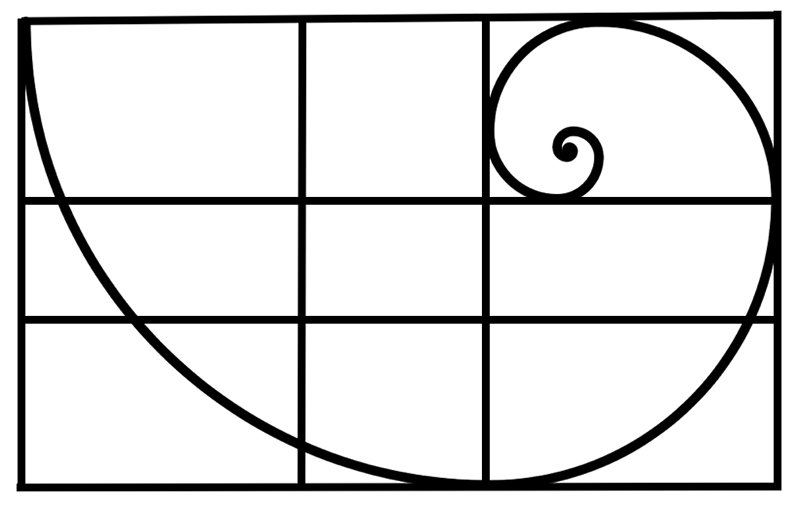
\includegraphics[width=.3\textwidth]{figures/chap4/figures/golden_ratio}
    \caption{The golden ratio}
    \label{c4:golden_ratio}
\end{figure}


\begin{figure}[ht!]
    \centering  
    \subfigure{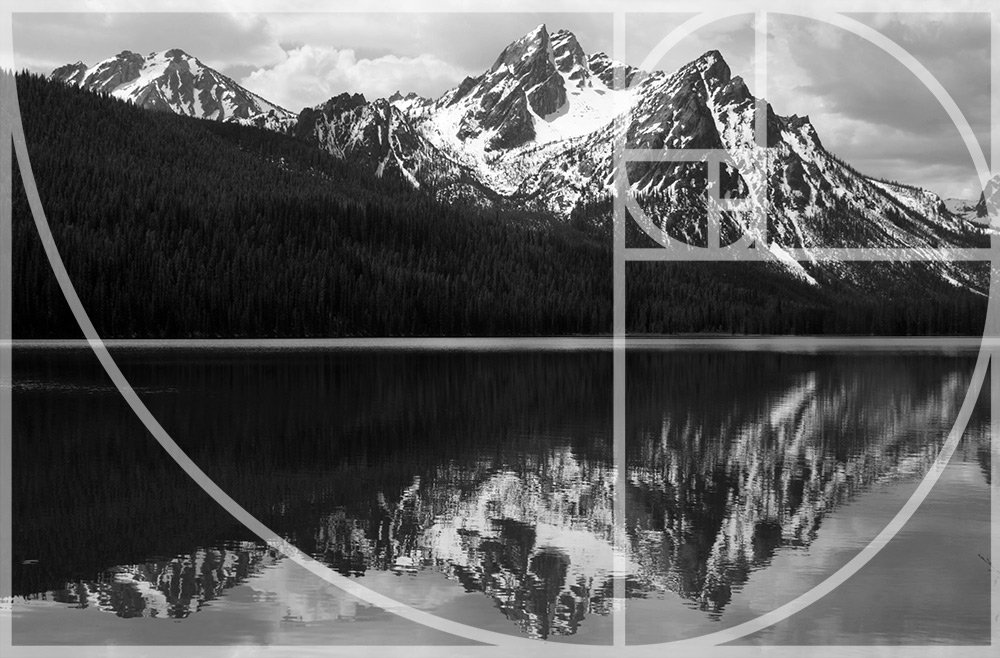
\includegraphics[width=.45\textwidth]{figures/chap4/figures/golden_adams}}
    \subfigure{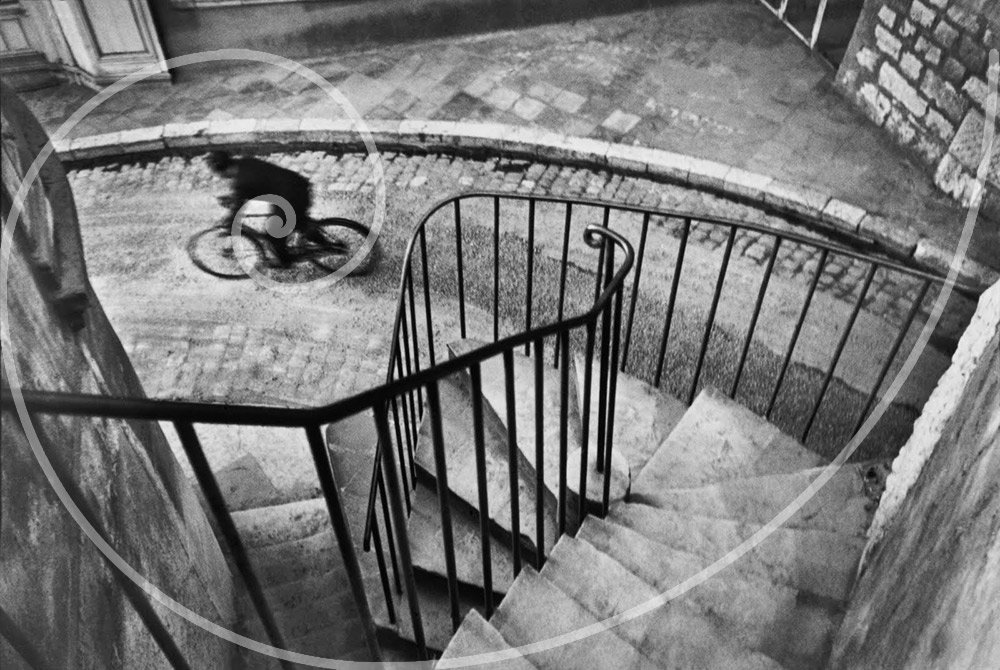
\includegraphics[width=.45\textwidth]{figures/chap4/figures/golden_brenson}}   
    \caption{Left: Ansel Adams, Right: Henri Cartier-Bresson}
    \label{c4:golden_photographer}
\end{figure}

The target image size for horizontal images is equal to (300,200) for horizontal images,equal to (200,300) for vertical images and equal to (400,400) for datasets with both orientations.
During image resize, \textit{inter area interpolation} were applied, to resample using pixel area relation. This technique offers moire-free results, a geometrical pattern produced in various digital imaging and computer graphics techniques due to undersampling.
To preserve the aspect ratio we have calculated the ratio of the target axis to the maximum reference image axis resolution. 
For an image that its original size is above or bellow the target ratio ($3/2$), the final outcome after the resize, will be a larger image which needs to get cropped or a smaller image which need to get padded with zeros.
The aforementioned transformation process is described in Algorithm~\ref{c4:algorithm}. Additionally, we have provided a meaning full representations of the transformed images in Figures~\ref{c4:horizontal_crop}-\ref{c4:square_transformation}.

\begin{algorithm}
\caption{Image transformation}
\label{c4:algorithm}
\begin{algorithmic}[1]
\Procedure {Resize\_Image}{$image$, $target.width$, $target.height$, $orientation$}
    \If{orientation == Horizontal}
        \State $ratio \leftarrow target.width/max(image.size) $
    \ElsIf{orientation == Vertical}  
        \State $ratio \leftarrow target.height/max(image.size) $
    \EndIf

    \State $new\_size \leftarrow [image.width*ratio, image.height*ratio]$
    \Comment {calculate new size}

    \State $new\_image \leftarrow resize(image, [new\_size.width, new\_size.height], \text{INTER\_AREA\_IP}) $
    \State
    \If{$new\_image.width \neq target.width$}
        \Comment {crop/pad $\rightarrow$ target width}
        \State $new\_image \leftarrow pad\_crop(new\_image, target.width)$
    \ElsIf{$new\_image.height \neq target.height$}
        \Comment {crop/pad $\rightarrow$ target height}
        \State $new\_image \leftarrow pad\_crop(new\_image, target.height)$
    \EndIf
\EndProcedure
\State
\Procedure {pad\_crop}{$image$, $target.width$}
    \If{image.width $>$ target.width}
        \Comment {Evenly Crop image}
        \State $rows\_to\_crop \leftarrow target.width - image.width$
        \State $split\_rows \leftarrow rows\_to\_crop$ \text{DIV} 2
        \If {rows\_to\_crop MOD 2 == 0}
            \State $new\_image \leftarrow image[width-split\_rows: split\_rows]$
        \Else \Comment {Rows to crop odd number, crop one more}
            \State $new\_image \leftarrow image[width-split\_rows: split\_rows+1]$
        \EndIf
    \Else
        \Comment {Evenly 0Pad image}
        \State $rows\_to\_pad \leftarrow target.width - image.width$
        \State $pad\_rows \leftarrow rows\_to\_pad$ \text{DIV} 2
        \If {rows\_to\_pad MOD 2 == 0}
            \State $new\_image \leftarrow$ PADDING0(image, $pad\_rows$)
        \Else \Comment {Rows to pad odd number, pad one more}
            \State $new\_image \leftarrow$ PADDING0(image, $pad\_rows+1$)
        \EndIf
    \EndIf
\EndProcedure
\end{algorithmic}
\end{algorithm}



\begin{figure}[ht!]
    \centering  
    \subfigure{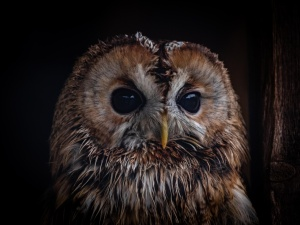
\includegraphics[width=.30\textwidth]{figures/chap4/photos/preprocessing/horizontal/crop/horizontal_resized_with_ratio}}
    \subfigure{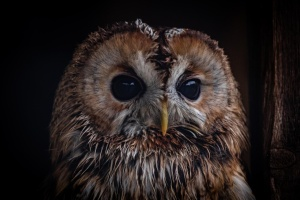
\includegraphics[width=.30\textwidth]{figures/chap4/photos/preprocessing/horizontal/crop/horizontal_resized_with_ratio_crop_y}}
    \subfigure{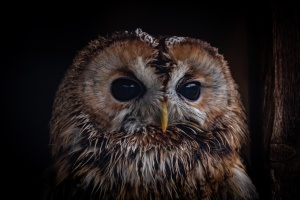
\includegraphics[width=.30\textwidth]{figures/chap4/photos/preprocessing/horizontal/crop/horizontal_resized_without_ratio}}
    \caption{Horizontal Crop, Left: Resized preserving ratio (325x200), Middle: Resized preserving ratio \& Crop to target (300,200), Right: Resized to target without preserving ratio}
    \label{c4:horizontal_crop}
\end{figure}

\begin{figure}[ht!]
    \centering  
    \subfigure{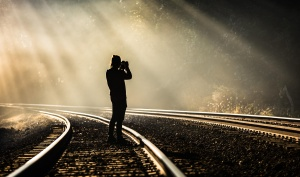
\includegraphics[width=.30\textwidth]{figures/chap4/photos/preprocessing/horizontal/pad/horizontal_resized_with_ratio}}
    \subfigure{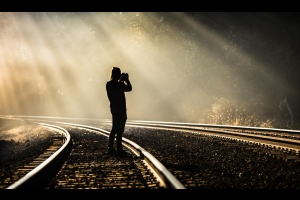
\includegraphics[width=.30\textwidth]{figures/chap4/photos/preprocessing/horizontal/pad/horizontal_resized_with_ratio_pad_y}}
    \subfigure{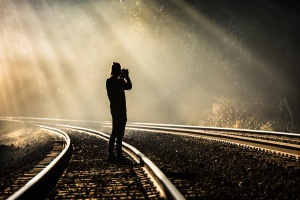
\includegraphics[width=.30\textwidth]{figures/chap4/photos/preprocessing/horizontal/pad/horizontal_resized_without_ratio}}
    \caption{Horizontal Pad, Left: Resized preserving ratio (300x177), Middle: Resized preserving ratio \& 0Pad to target (300,200), Right: Resized to target without preserving ratio}
    \label{c4:horizontal_pad}
\end{figure}


\begin{figure}[ht!]
    \centering  
    \subfigure{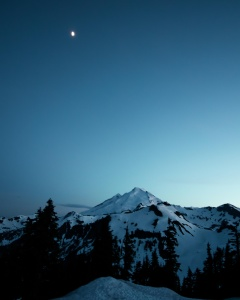
\includegraphics[width=.20\textwidth]{figures/chap4/photos/preprocessing/vertical/crop/vertical_resized_with_ratio}}
    \subfigure{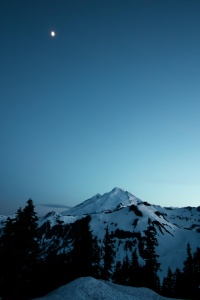
\includegraphics[width=.20\textwidth]{figures/chap4/photos/preprocessing/vertical/crop/vertical_resized_with_ratio_crop_x}}
    \subfigure{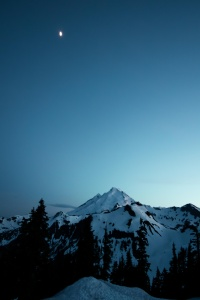
\includegraphics[width=.20\textwidth]{figures/chap4/photos/preprocessing/vertical/crop/vertical_resized_without_ratio}}
    \caption{Vertical Crop, Left: Resized preserving ratio (240x300), Middle: Resized preserving ratio \& Crop to target (200,300), Right: Resized to target without preserving ratio}
    \label{c4:vertical_crop}
\end{figure}

\begin{figure}[ht!]
    \centering  
    \subfigure{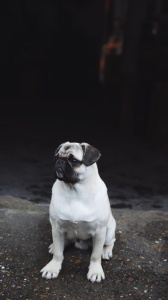
\includegraphics[width=.20\textwidth]{figures/chap4/photos/preprocessing/vertical/pad/vertical_resized_with_ratio}}
    \subfigure{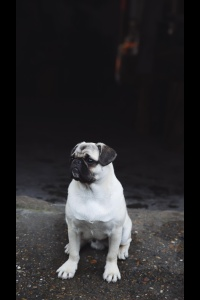
\includegraphics[width=.20\textwidth]{figures/chap4/photos/preprocessing/vertical/pad/vertical_resized_with_ratio_pad_x}}
    \subfigure{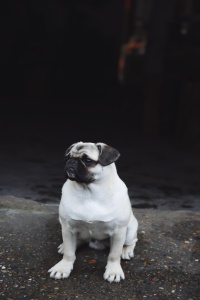
\includegraphics[width=.20\textwidth]{figures/chap4/photos/preprocessing/vertical/pad/vertical_resized_without_ratio}}
    \caption{Vertical Pad, Left: Resized preserving ratio (168x300), Middle: Resized preserving ratio \& 0Pad to target (200,300), Right: Resized to target without preserving ratio}
    \label{c4:vertical_pad}
\end{figure}

\begin{figure}[ht!]
    \centering  
    \subfigure{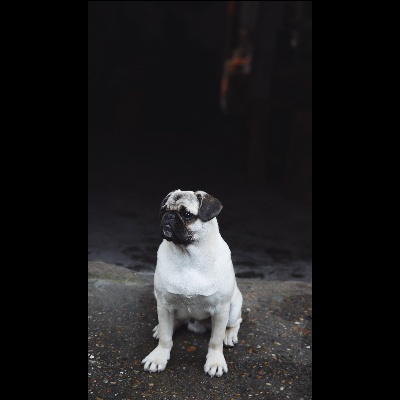
\includegraphics[width=.3\textwidth]{figures/chap4/photos/preprocessing/square/1}}
    \subfigure{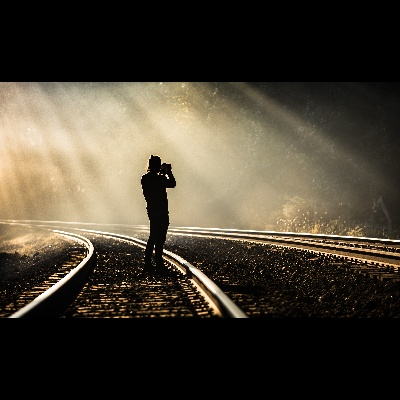
\includegraphics[width=.3\textwidth]{figures/chap4/photos/preprocessing/square/2}}
    \subfigure{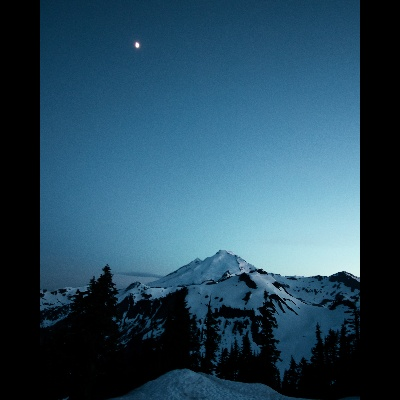
\includegraphics[width=.3\textwidth]{figures/chap4/photos/preprocessing/square/3}}
    \caption{Dataset in squarified transformation for both orientations to 400x400 by 0Padding}
    \label{c4:square_transformation}
\end{figure}


\section{Exploratory Data Analysis}
\label{c4:eda}

The first step to approach an unknown and recently published dataset, could be done with an exploratory data analysis (EDA). Its purpose is to perform a critical process to discover patterns, eliminate data anomalies and summarize main dataset's characteristics with the help of graphical representations to uncover certain aspects.

In a first level exploration the goal is to identify and comprehend the supplementary data(metadata) aside from images. We are looking for  identifier columns and levels for a categorical variable. In order to achieve that, we project the list of the available feature columns, perform a data cleansing process and create uni-variate histograms.

The scope beyond first level analysis, is to manually construct a labelled dataset relying solely on EXIF features. By applying a binning strategy based on photography domain knowledge, we aim to create data bins for each of the features in order to assign an appropriate label.
Uni-variate binning will aid us to form an initial hypothesis and setup a dataset driven problem that will be used as an indicator for a specific photography style classification problem.

Complementary to the EXIF-based labelled dataset, using the insights from the EDA, we have manually labelled a dataset based on the qualitative characteristics of a certain photography style.
The aforementioned process is depicted in Figure~\ref{c4:etl}.

\begin{figure}[ht!]
    \centering  
    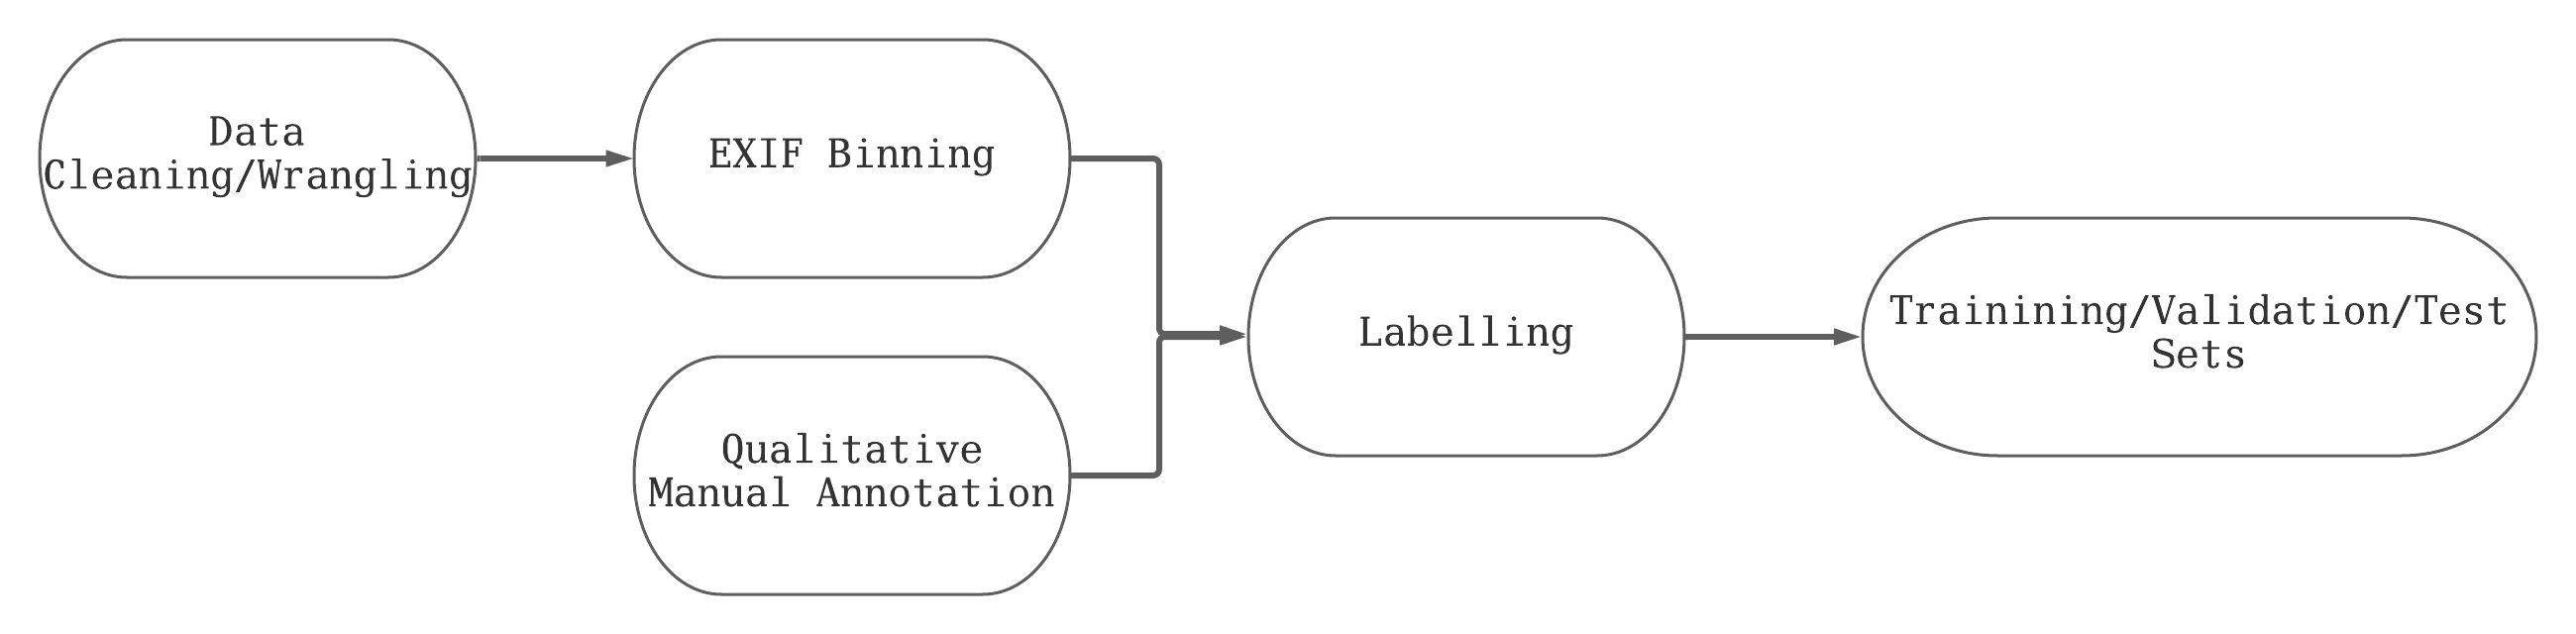
\includegraphics[width=.9\textwidth]{figures/chap4/etl}
    \caption{ETL process}
    \label{c4:etl}
\end{figure}

\subsection{Data Cleaning}
\label{c4:data_cleaning}

\textbf{Photos} dataset is comprised of \textbf{25318} samples in total with more than 15 features and photography metadata, that only a few can be considered as features or candidate labels.
In our case study, we focus only on EXIF(exchangeable image file format) metadata such \textbf{ISO}, the digital sensor's sensitivity, lens \textbf{aperture} value, lens \textbf{focal length} and shutter's \textbf{exposure time} as they represent the camera settings when a picture is captured. Additionally we have included \textbf{width} and \textbf{height} as they denote the picture's orientation.
The features we kept are shown in Table~\ref{c4:unsplash_feature_table}.

\begin{table}[ht!]
\centering
\begin{tabular}{|l|l|}
\hline
 \textbf{Feature} & \textbf{Description}  \\ \hline
 photo\_id  & Image filename  \\ \hline
 photo\_width & Width in pixels \\ \hline
 photo\_height & Height in pixels  \\ \hline
 photo\_aspect\_ratio & Photo aspect ratio \\ \hline
 exif\_iso & ISO setting(EXIF) \\ \hline
 exif\_aperture\_value & Aperture setting(EXIF) \\ \hline
 exif\_focal\_length & Focal length setting(EXIF) \\ \hline
 exif\_exposure\_time & Exposure time settings(EXIF)  \\ \hline
\end{tabular}
\caption{Table with Unsplash dataset metadata \& features}
\label{c4:unsplash_feature_table}
\end{table}

Any dataset collected from the web comes with distorted and noisy information which can negatively affect the analysis. 
A data mining process is required prior to any algorithm application, to increase consistency and interpretability of the studying data.

%% Cleaning
We implemented a data cleaning/wrangling process on EXIF feature values, to eliminate samples with \textit{NaN} entries and align each feature value range to a homogeneous format.
Data wrangling process, eliminated and corrected values with incoherent format e.g. for the case of aperture values, $1,8\rightarrow1.6$, f/5.6$\rightarrow$5.6, $180s \rightarrow 180$ and structural errors e.g. \textit{undef,Inf,inf,18-55mm}$\rightarrow$\textit{NaN}. Removing \textit{NaN} values we ended up with \textbf{21,445} working examples.

Next, we present a family of plots related with EXIF values distribution concerning both of the picture orientations in Figures~\ref{c4:all_dof_iso_values} and~\ref{c4:all_focal_exposure_values}.

%In terms of completion and coherence, we provide the same family of distributions for horizontal pictures in~\ref{c4:horizontal_values_distribution}, and vertical pictures~\ref{c4:vertical_values_distribution} respectively.

\begin{figure}[ht!]
    \centering  
    \subfigure[Aperture]{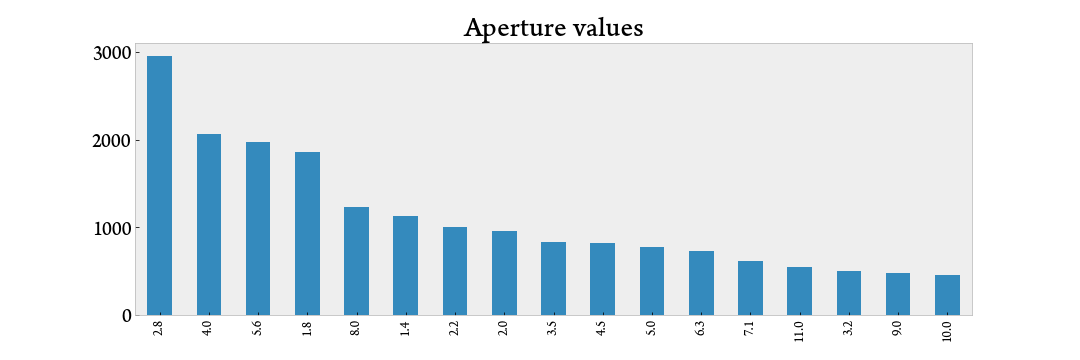
\includegraphics[width=.9\textwidth]{figures/chap4/exif/all/aperture_values}}
    \subfigure[ISO]{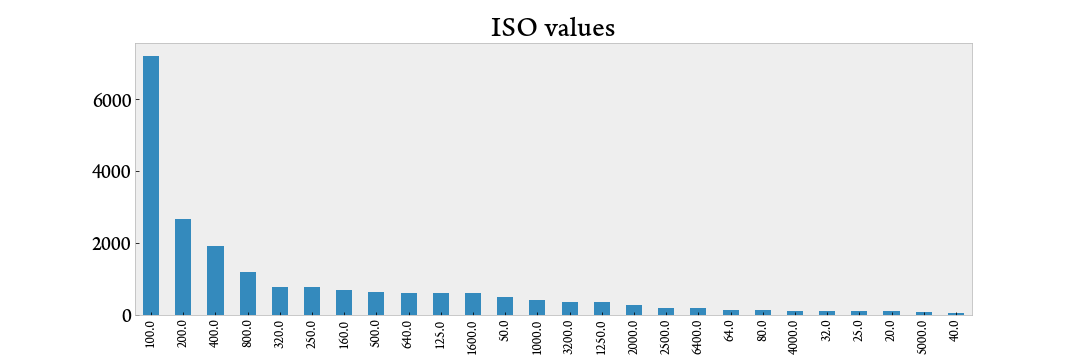
\includegraphics[width=.9\textwidth]{figures/chap4/exif/all/iso_values}}
    \caption{Horizontal$+$Vertical Aperture/ISO value distribution}
    \label{c4:all_dof_iso_values}
\end{figure}

It is observed that a large number of pictures are captured in middle to low aperture settings. Most photographers, choose these specific settings as most of the consumer lenses tend to be more sharper, with significant amount of Depth of Field separation from the subject.
Also, most of the captures are set in the lowest ISO values which means that images are free of natural noise that could be introduced from the camera sensor.

\begin{figure}[ht!]
    \centering  
    \subfigure{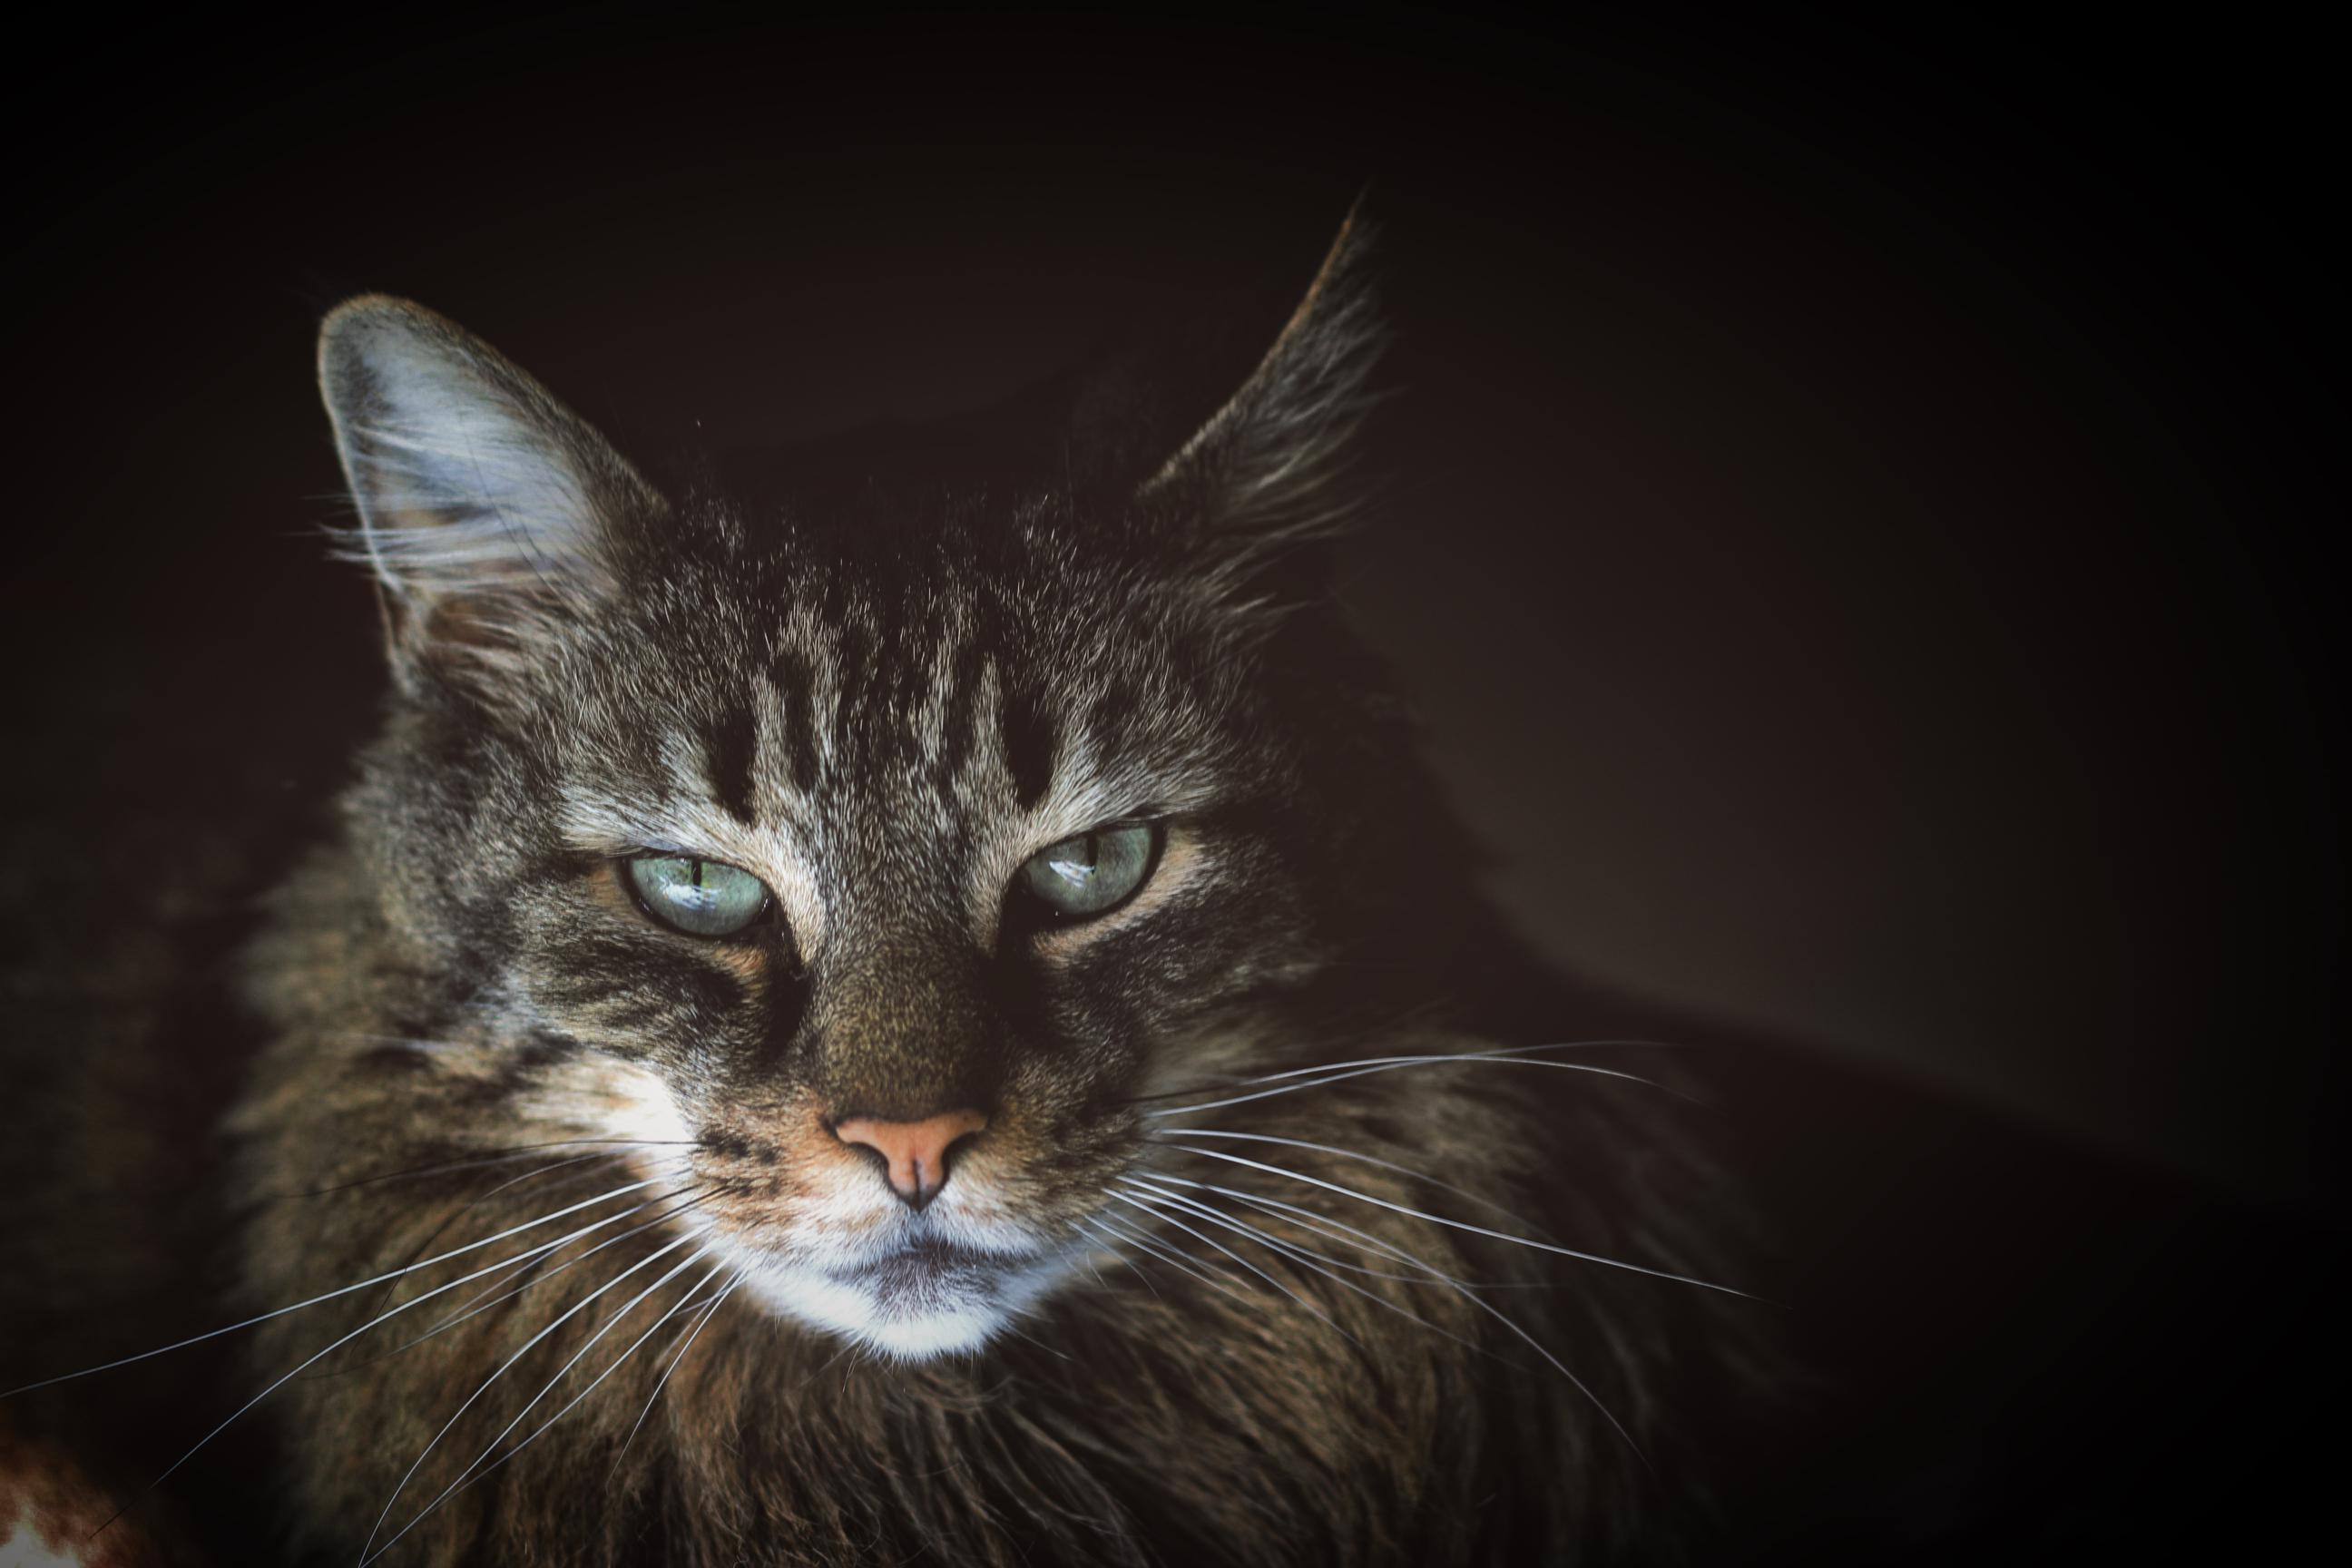
\includegraphics[width=.3\textwidth]{figures/chap4/photos/wideopen/1}}
    \subfigure{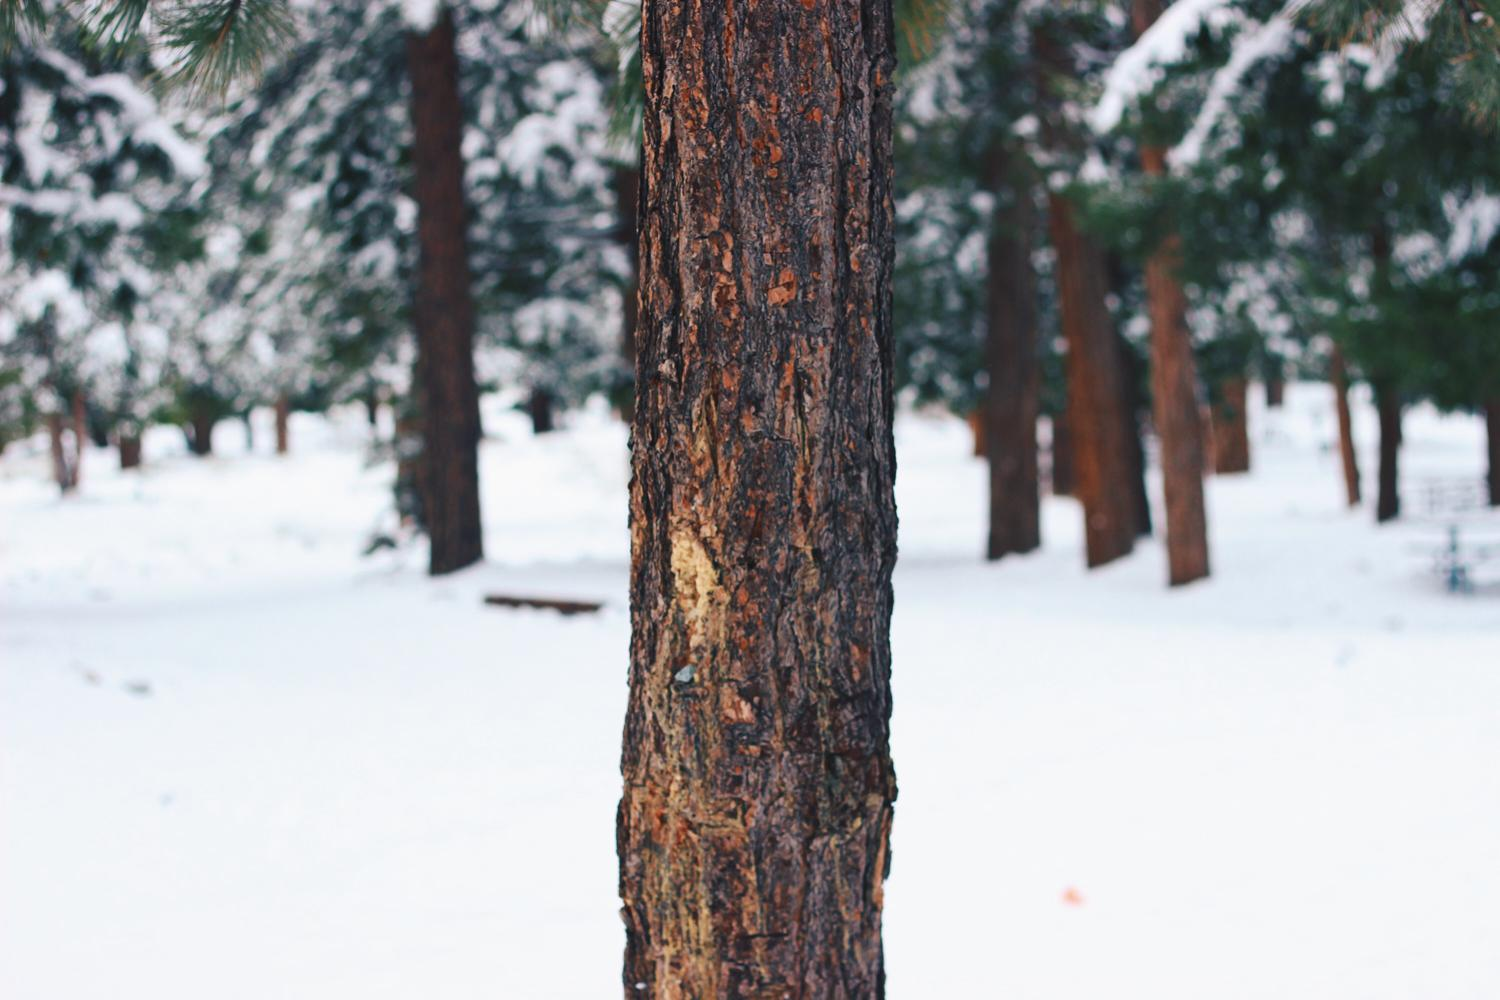
\includegraphics[width=.3\textwidth]{figures/chap4/photos/wideopen/2}}
    \subfigure{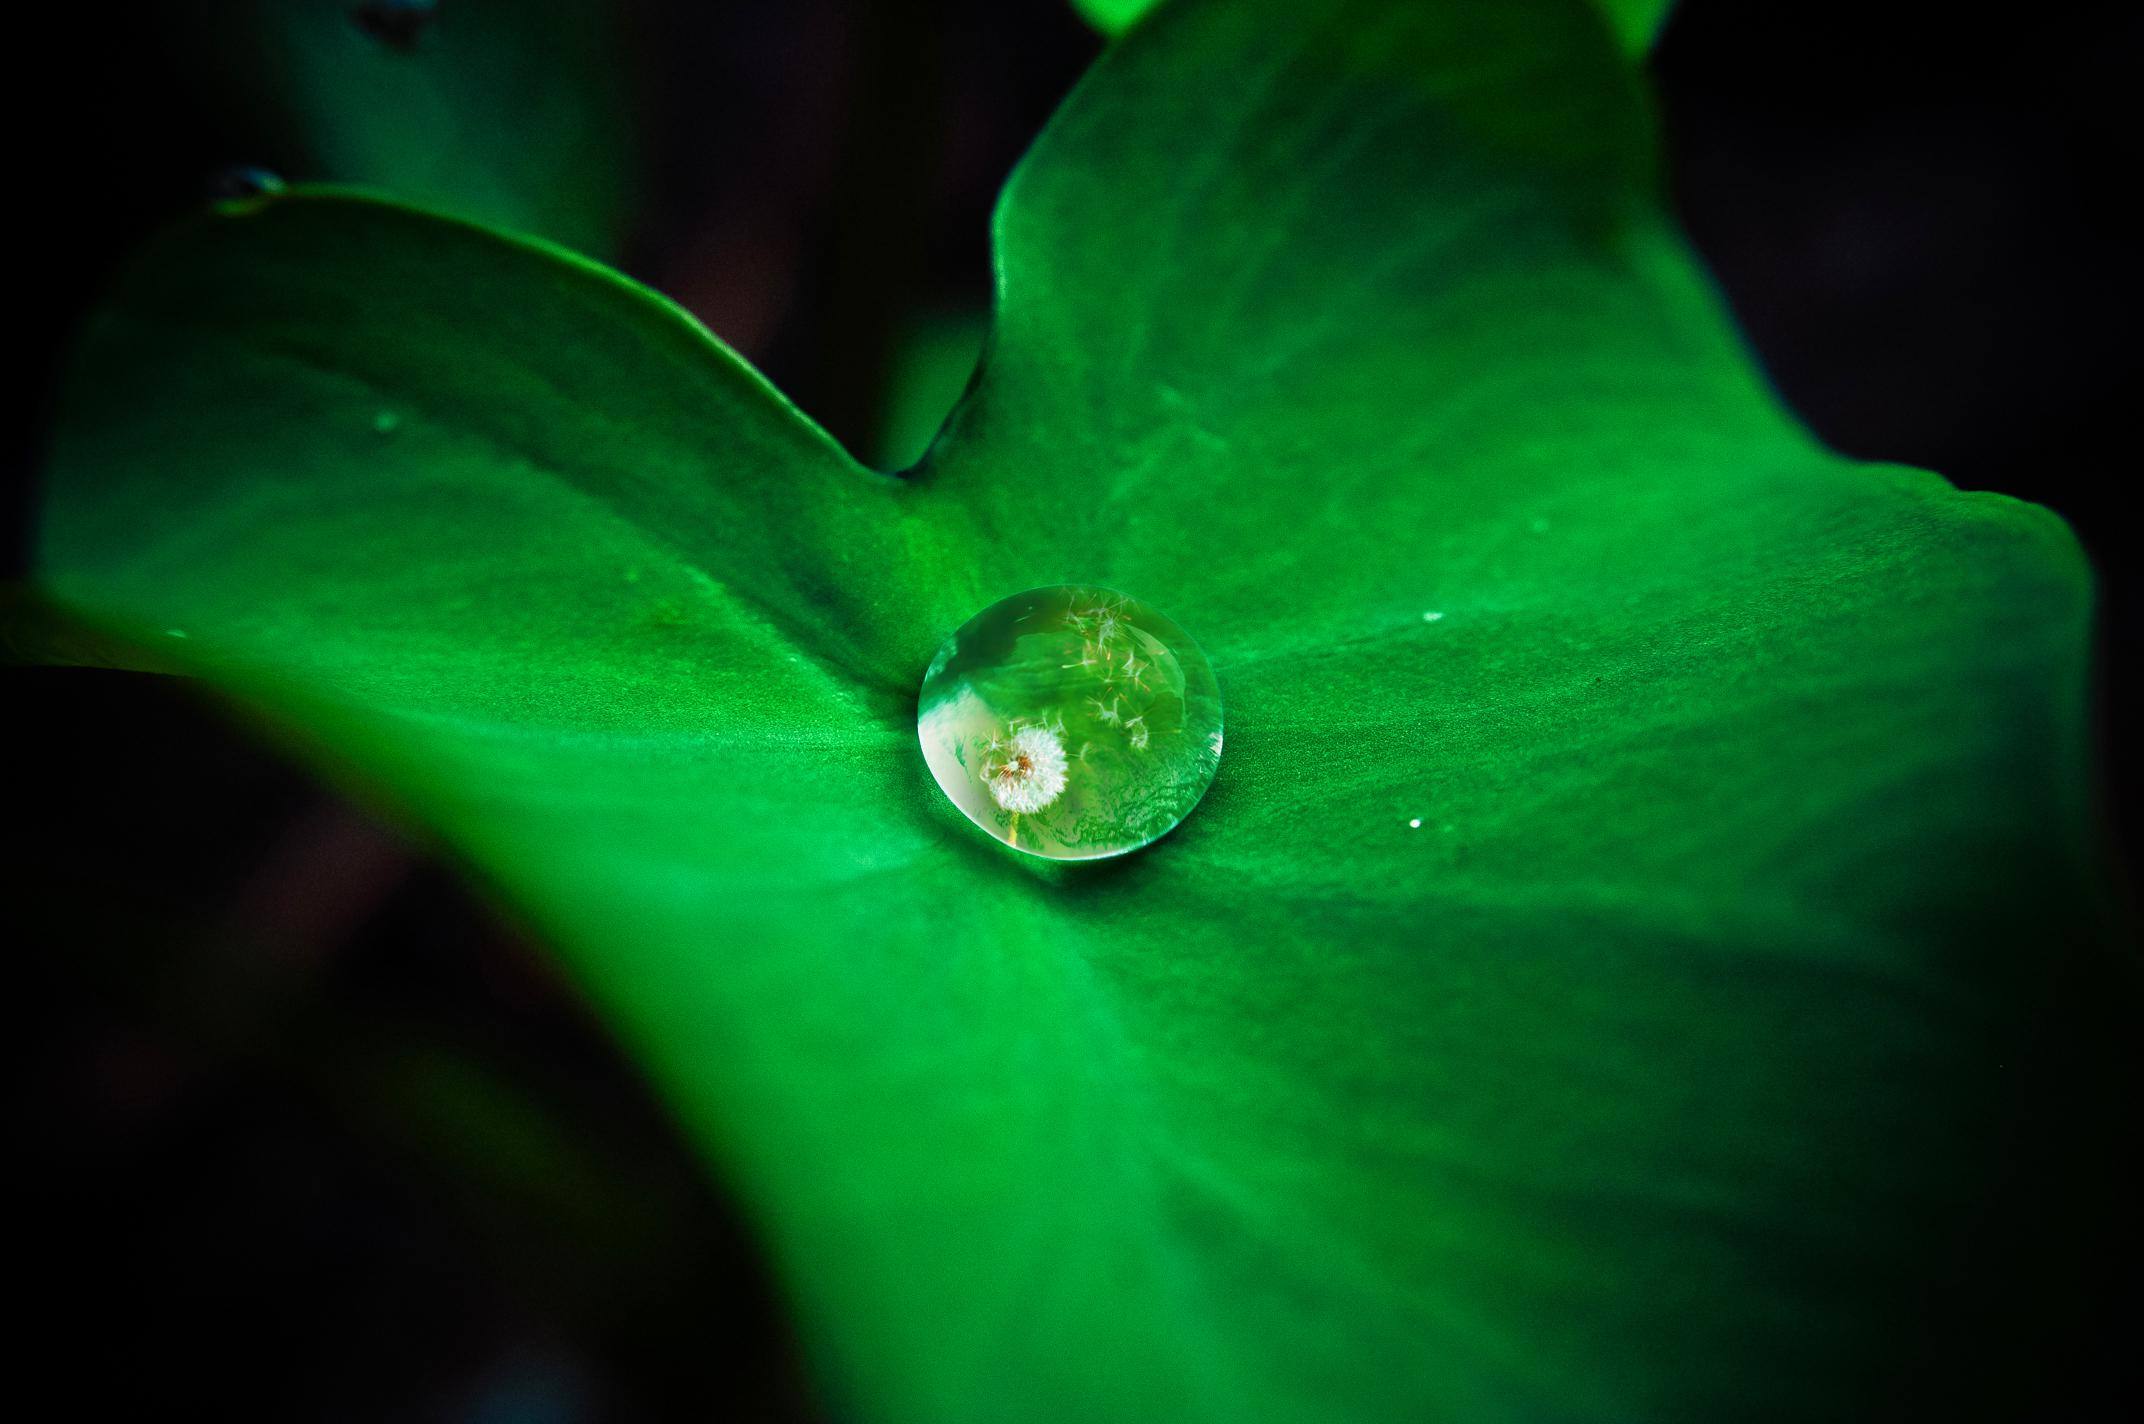
\includegraphics[width=.3\textwidth]{figures/chap4/photos/wideopen/3}}    
    \caption{Captures in $2.8$ and $5.6$(leaf) aperture setting}
    \label{c4:bokeh_captures}
\end{figure}

\begin{figure}[ht!]
    \centering  
    \subfigure{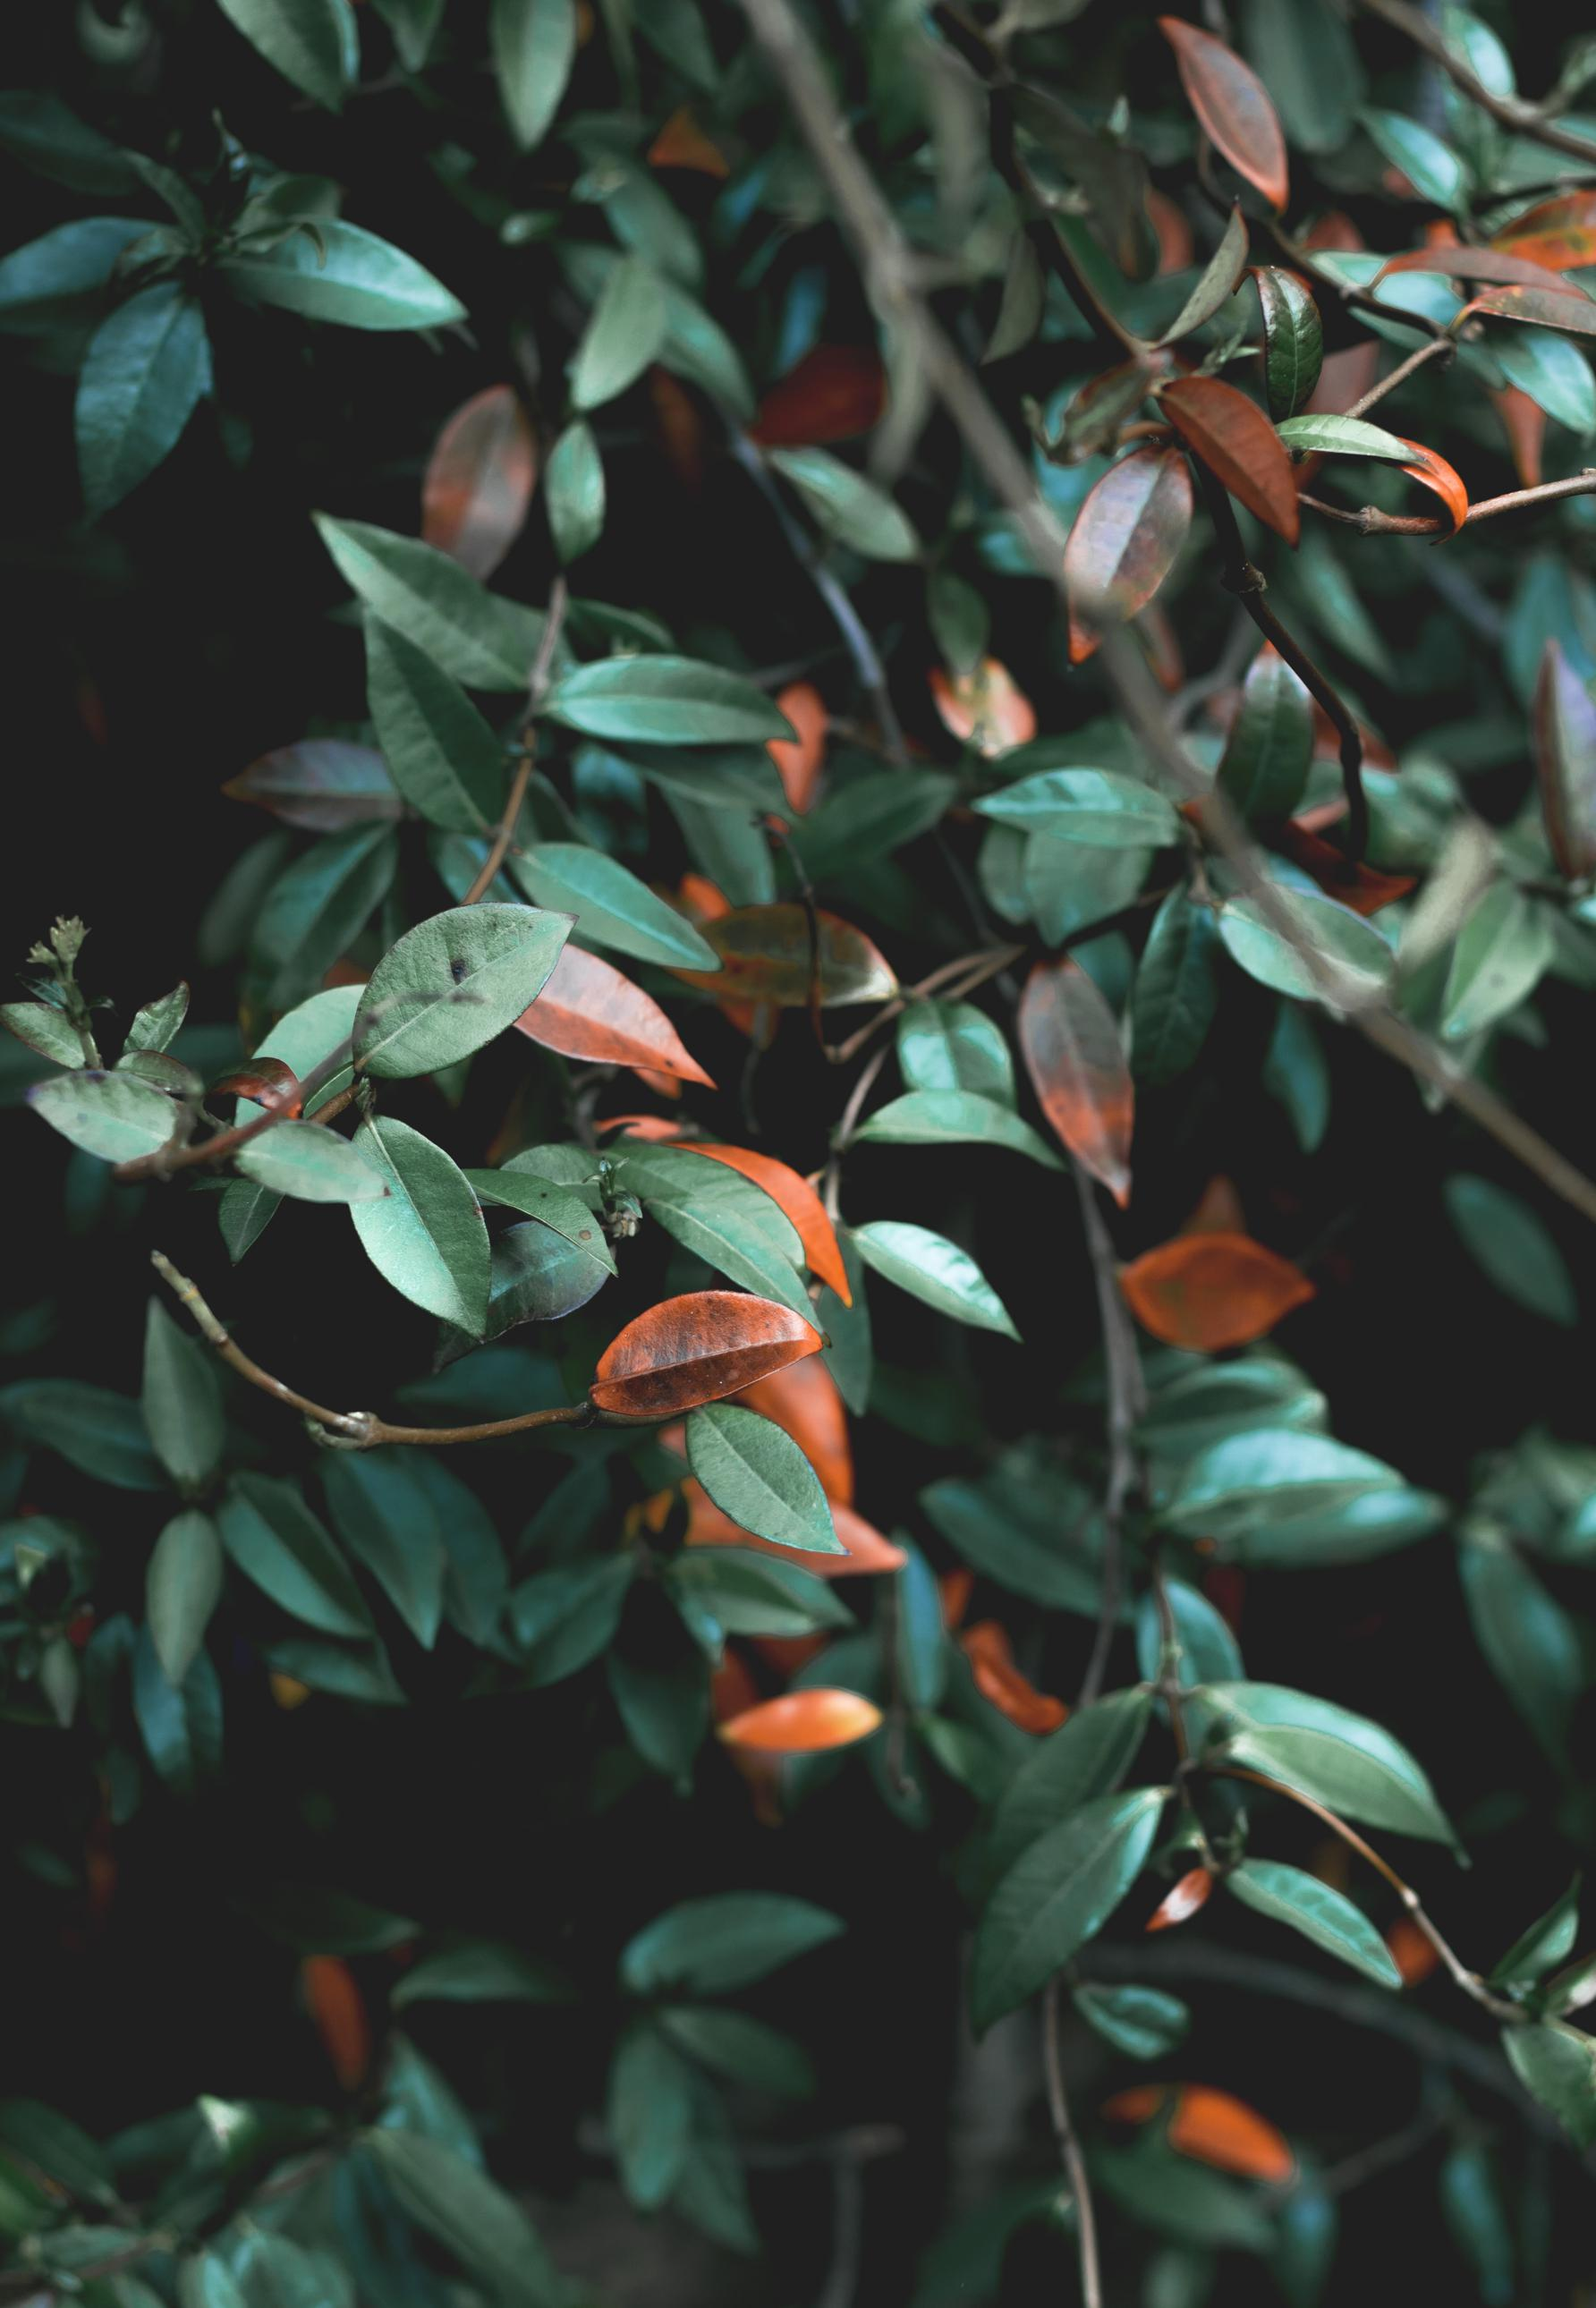
\includegraphics[width=.3\textwidth]{figures/chap4/photos/iso/1}}
    \subfigure{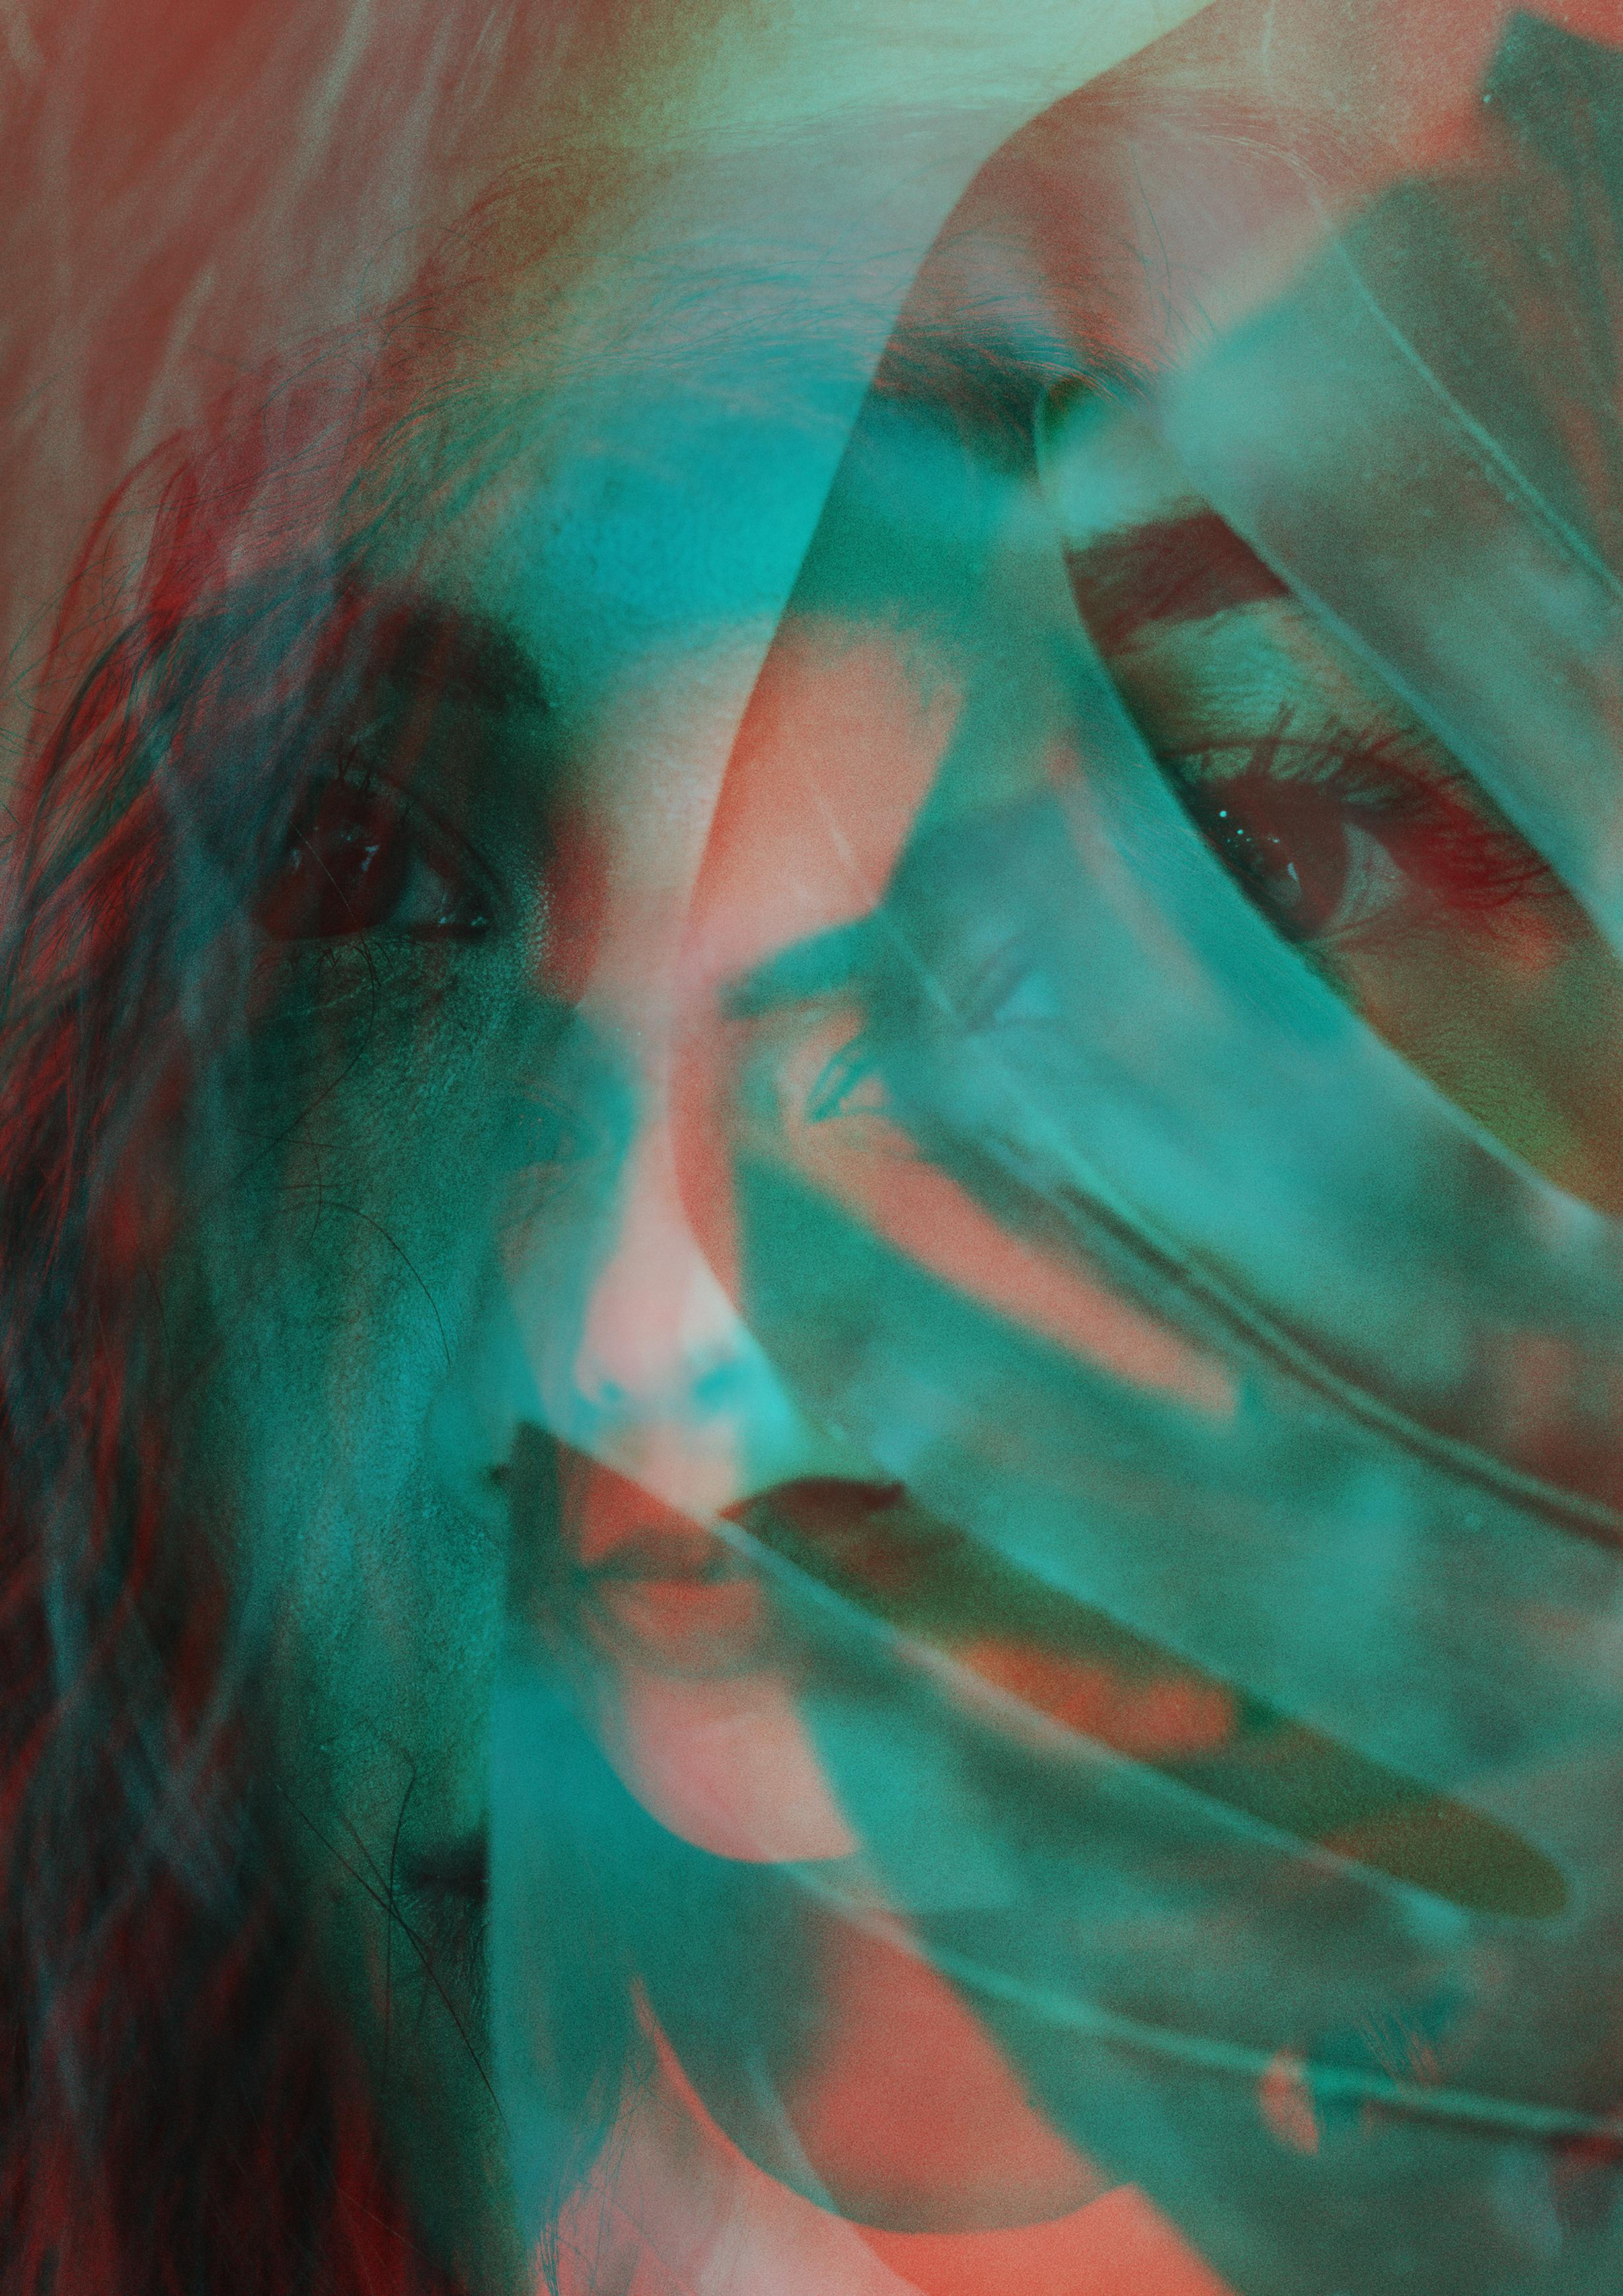
\includegraphics[width=.3\textwidth]{figures/chap4/photos/iso/2}}
    \caption{Captures in 100 and 5000 ISO setting}
    \label{c4:iso_captures}
\end{figure}


\begin{figure}[ht!]
    \centering  
    \subfigure[Focal Length]{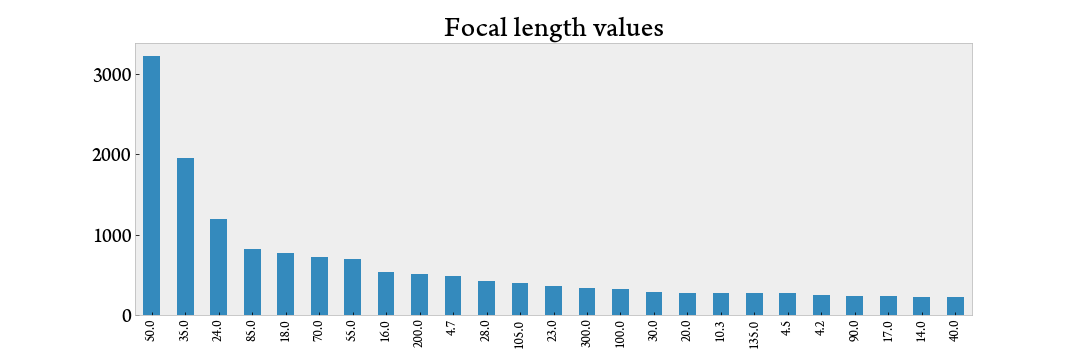
\includegraphics[width=.9\textwidth]{figures/chap4/exif/all/focal_values}}
    \subfigure[Exposure]{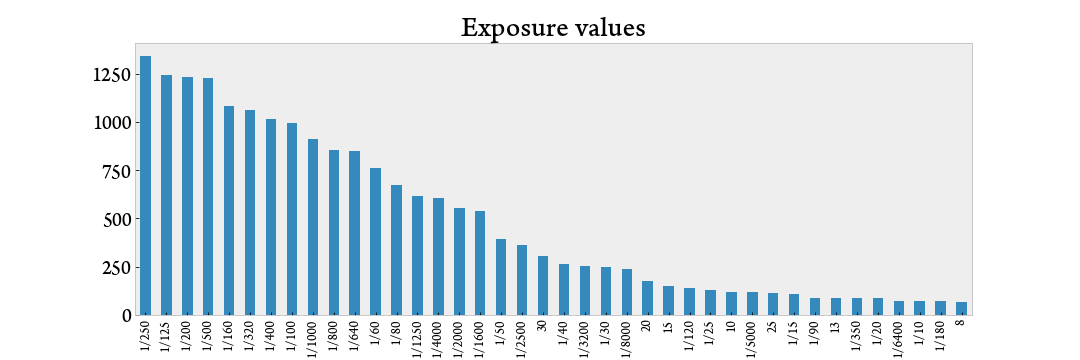
\includegraphics[width=.9\textwidth]{figures/chap4/exif/all/exposure_values}}
    \caption{Horizontal$+$Vertical Focal Length/Exposure value distribution}
    \label{c4:all_focal_exposure_values}
\end{figure}

Concerning focal length, most of the pictures are captured with 50mm lens, the most usual prime lens type that offers the closer to the human eye, feel in the visual field. In the same neighborhood, 35mm and 24mm lenses are used, types for general purpose shooting. These are wide angle enough to get the bigger picture but not so wide to lose the subject. Less of the captures can be considered as portraits in 85mm or more, while the rest bellow 24mm for landscape photography.
Exposure values are most of them in the typical general purpose range, fast enough to capture or even freeze any moving object while a few captures can be considered as long exposure shots.

\begin{figure}[ht!]
    \centering  
    \subfigure{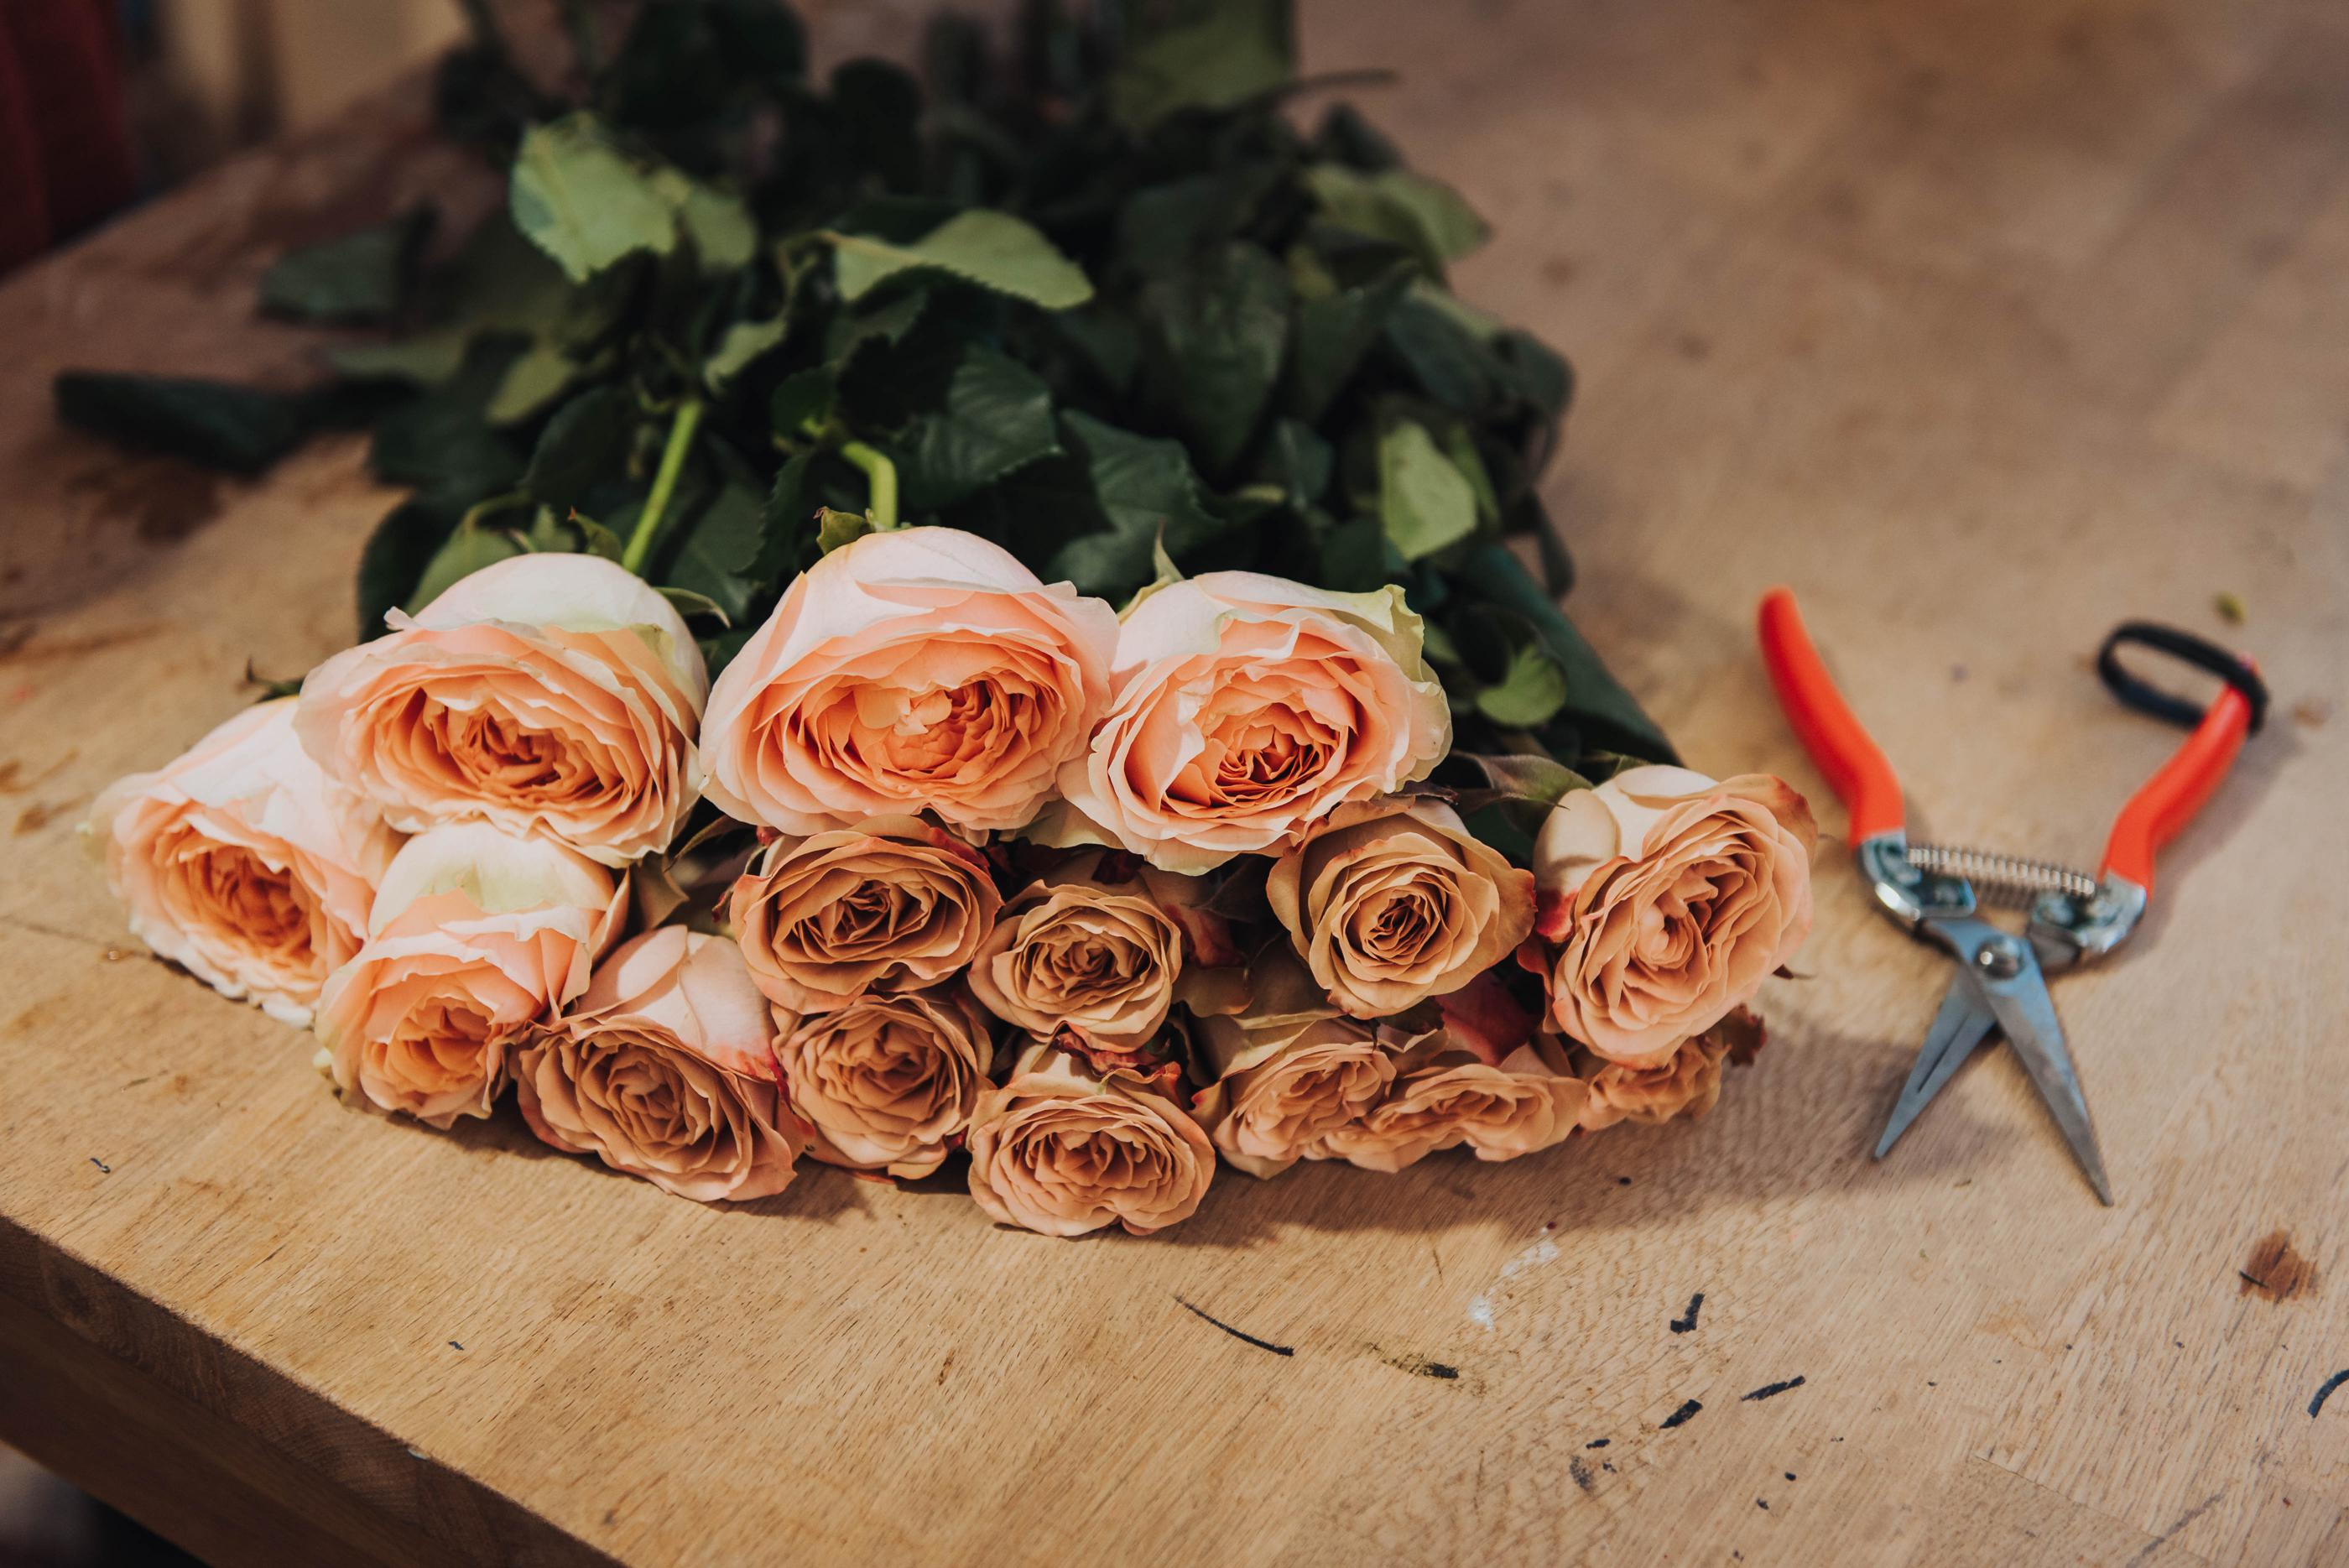
\includegraphics[width=.3\textwidth]{figures/chap4/photos/50/1}}
    \subfigure{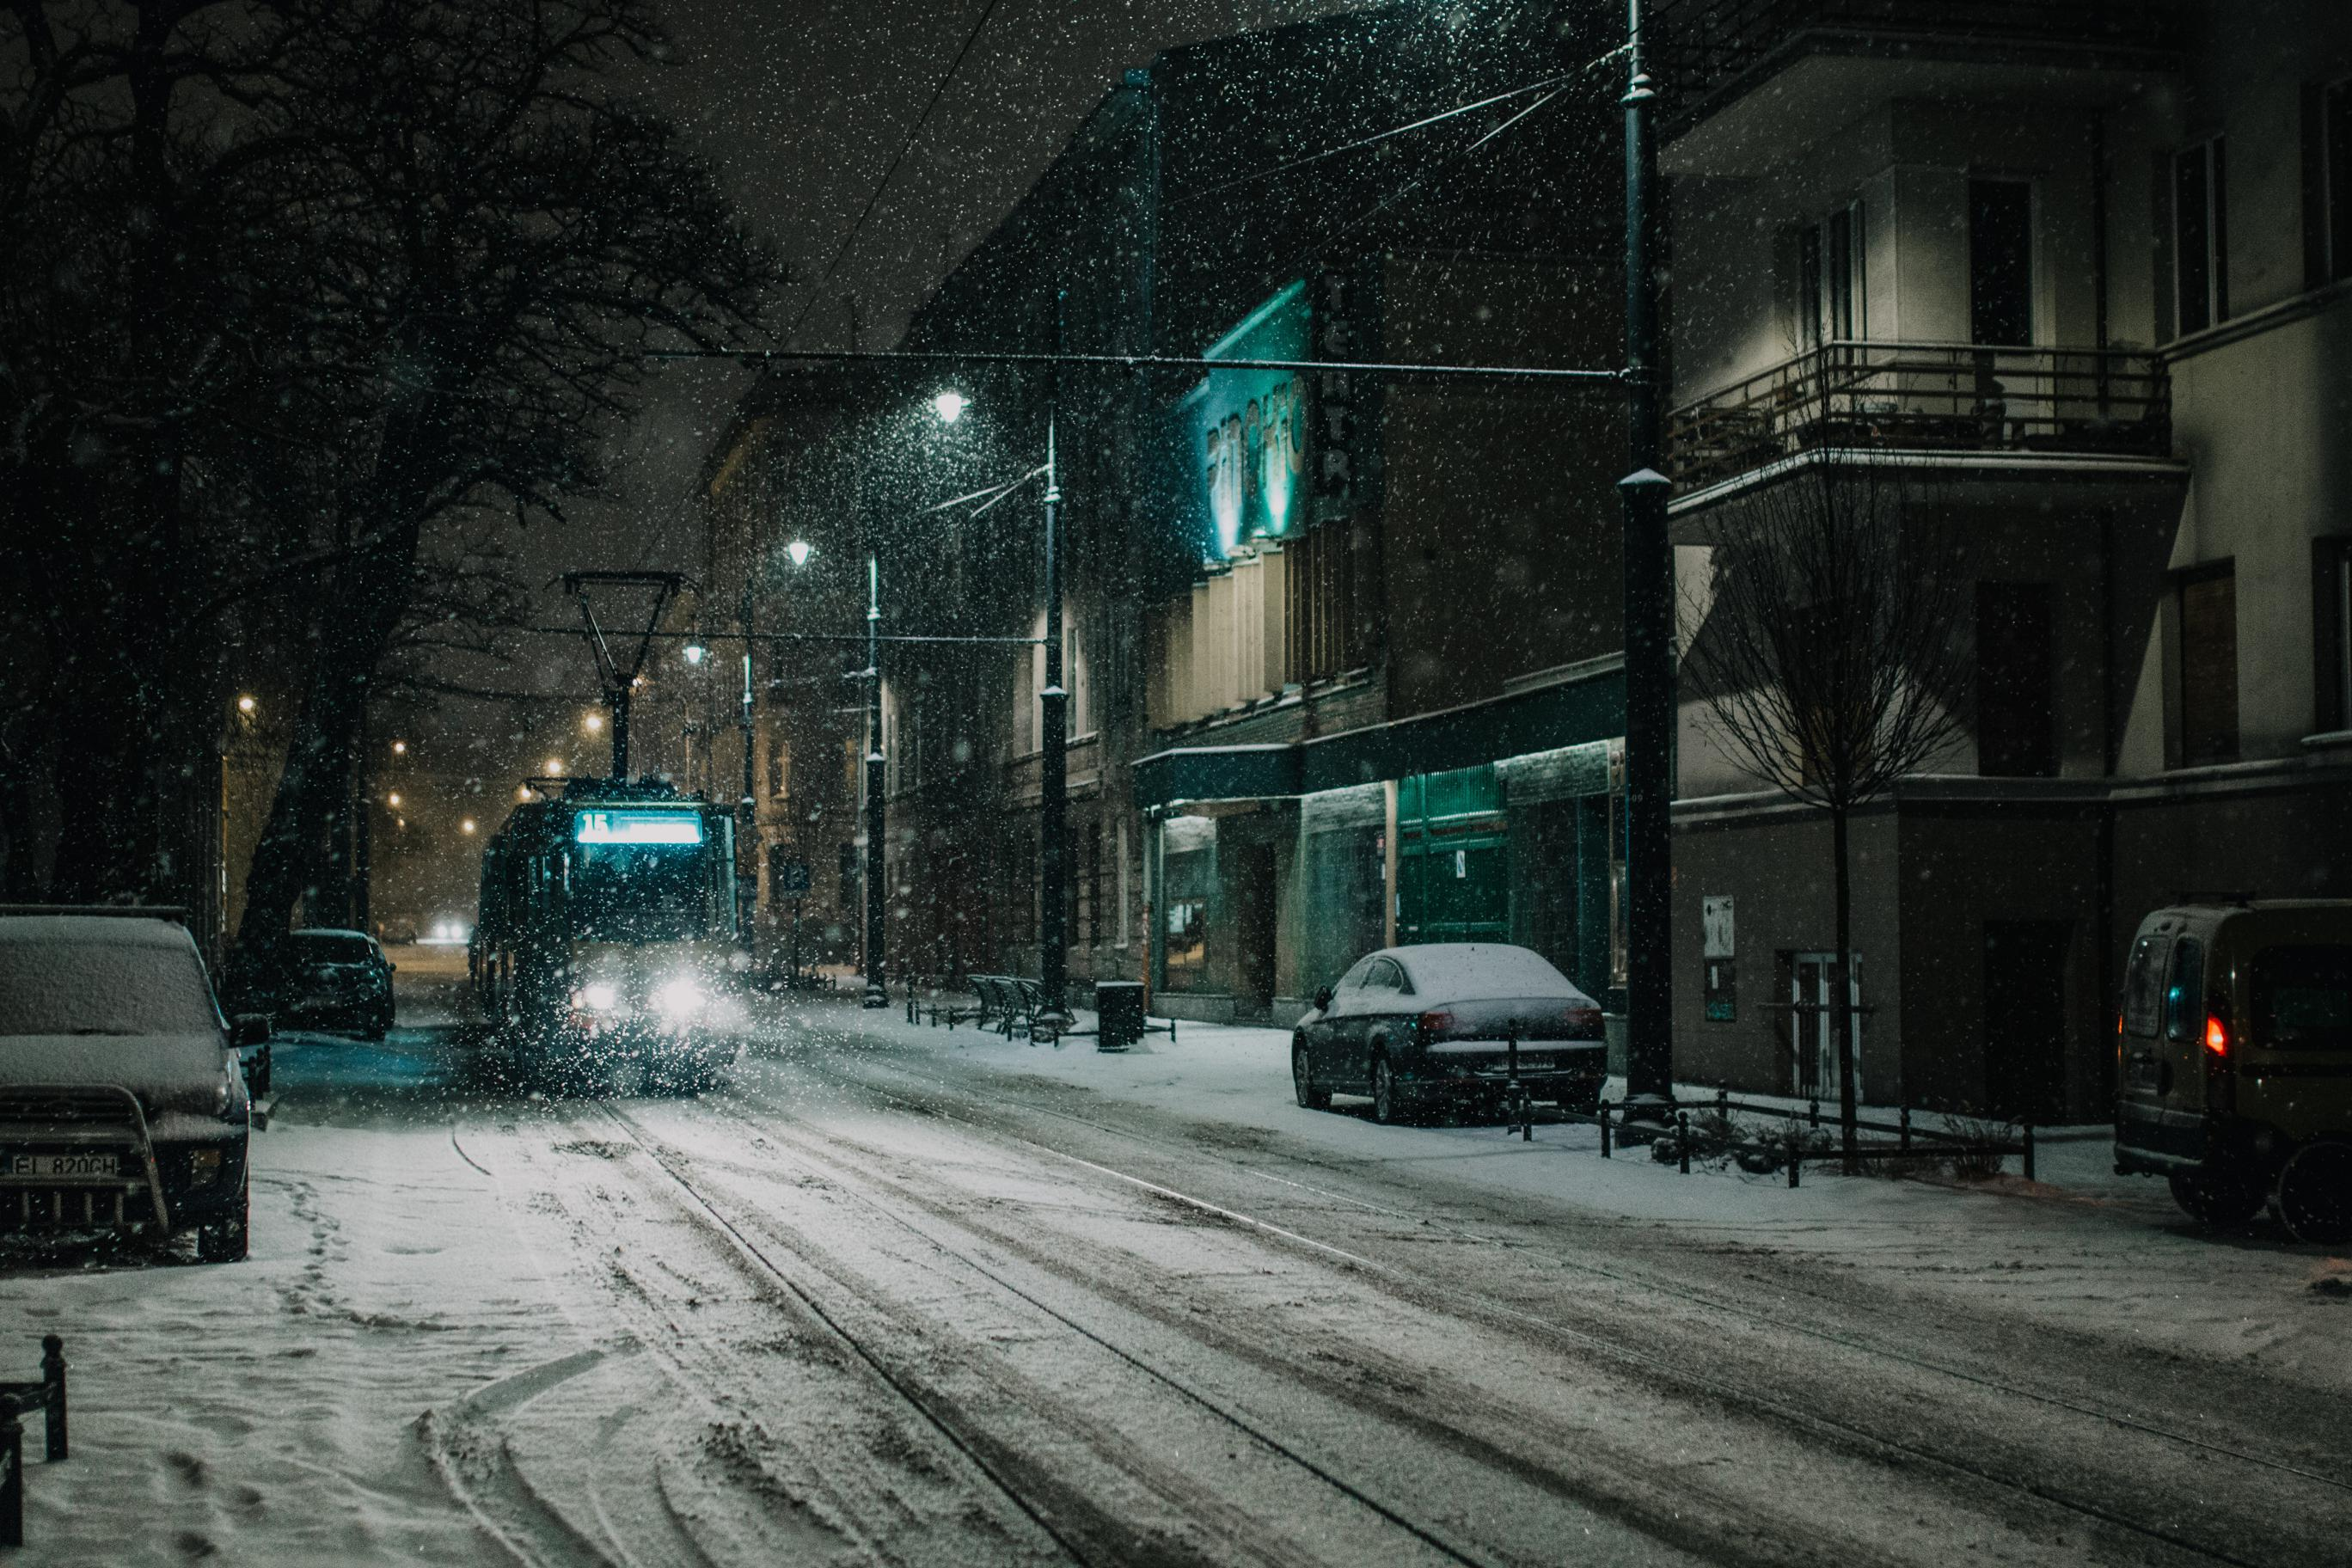
\includegraphics[width=.3\textwidth]{figures/chap4/photos/50/2}}
    \caption{Captures in $50$mm and $35$mm}
    \label{c4:focal_captures}
\end{figure}


\begin{figure}[ht!]
    \centering  
    \subfigure[]{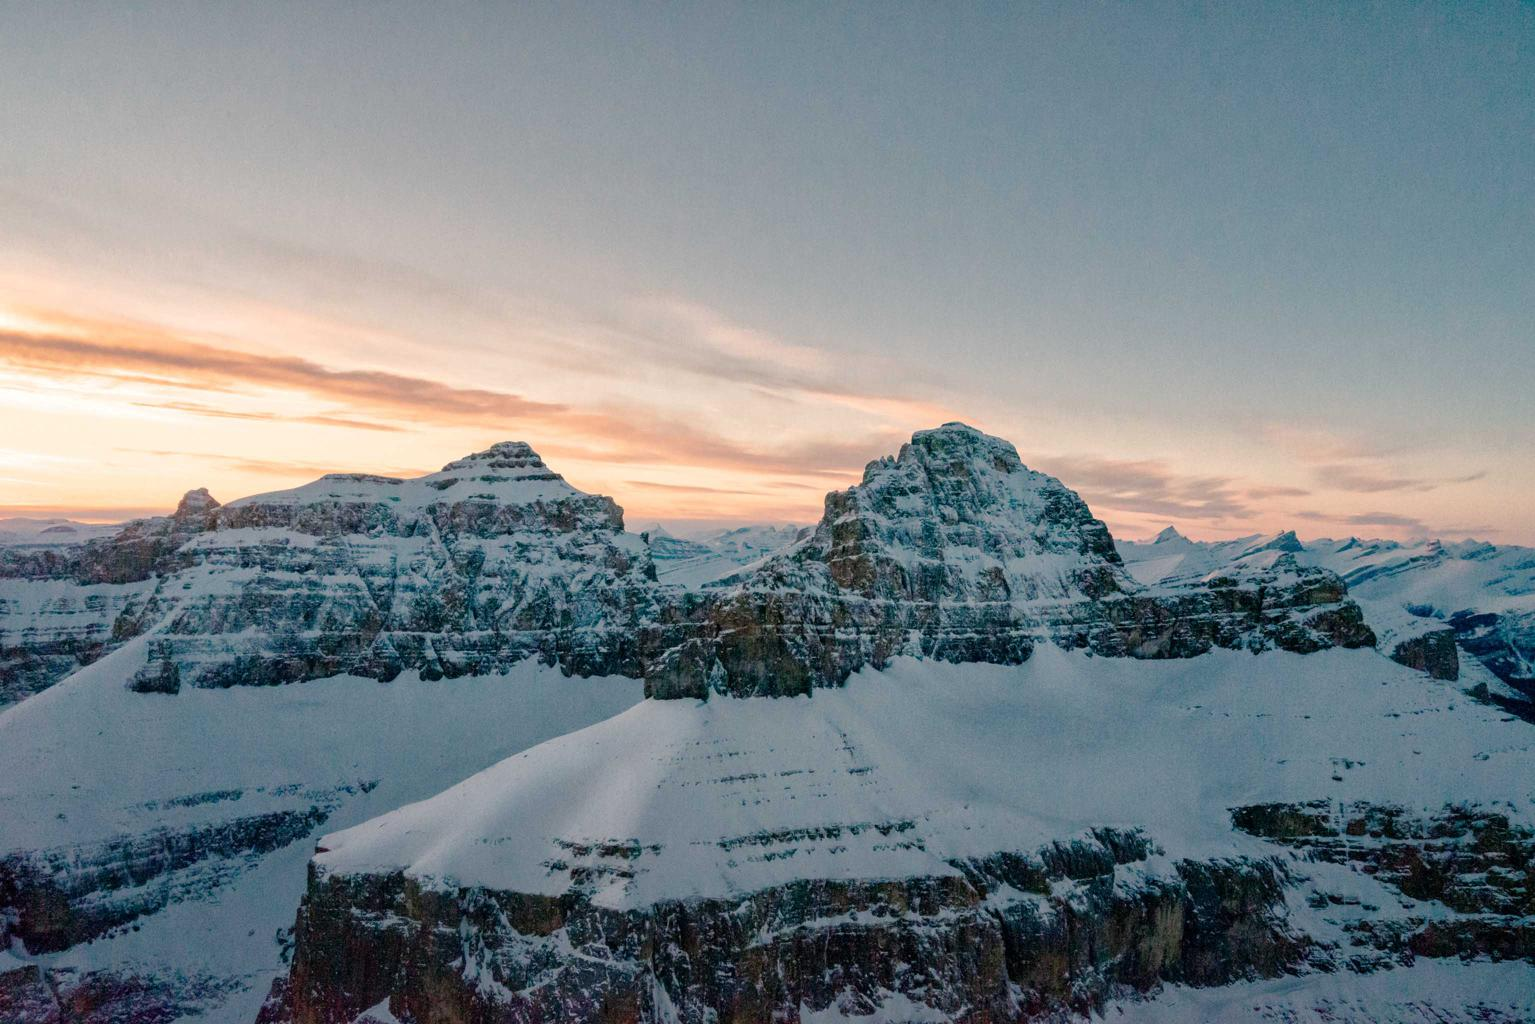
\includegraphics[width=.2\textwidth]{figures/chap4/photos/highshutter/1}}
    \subfigure[]{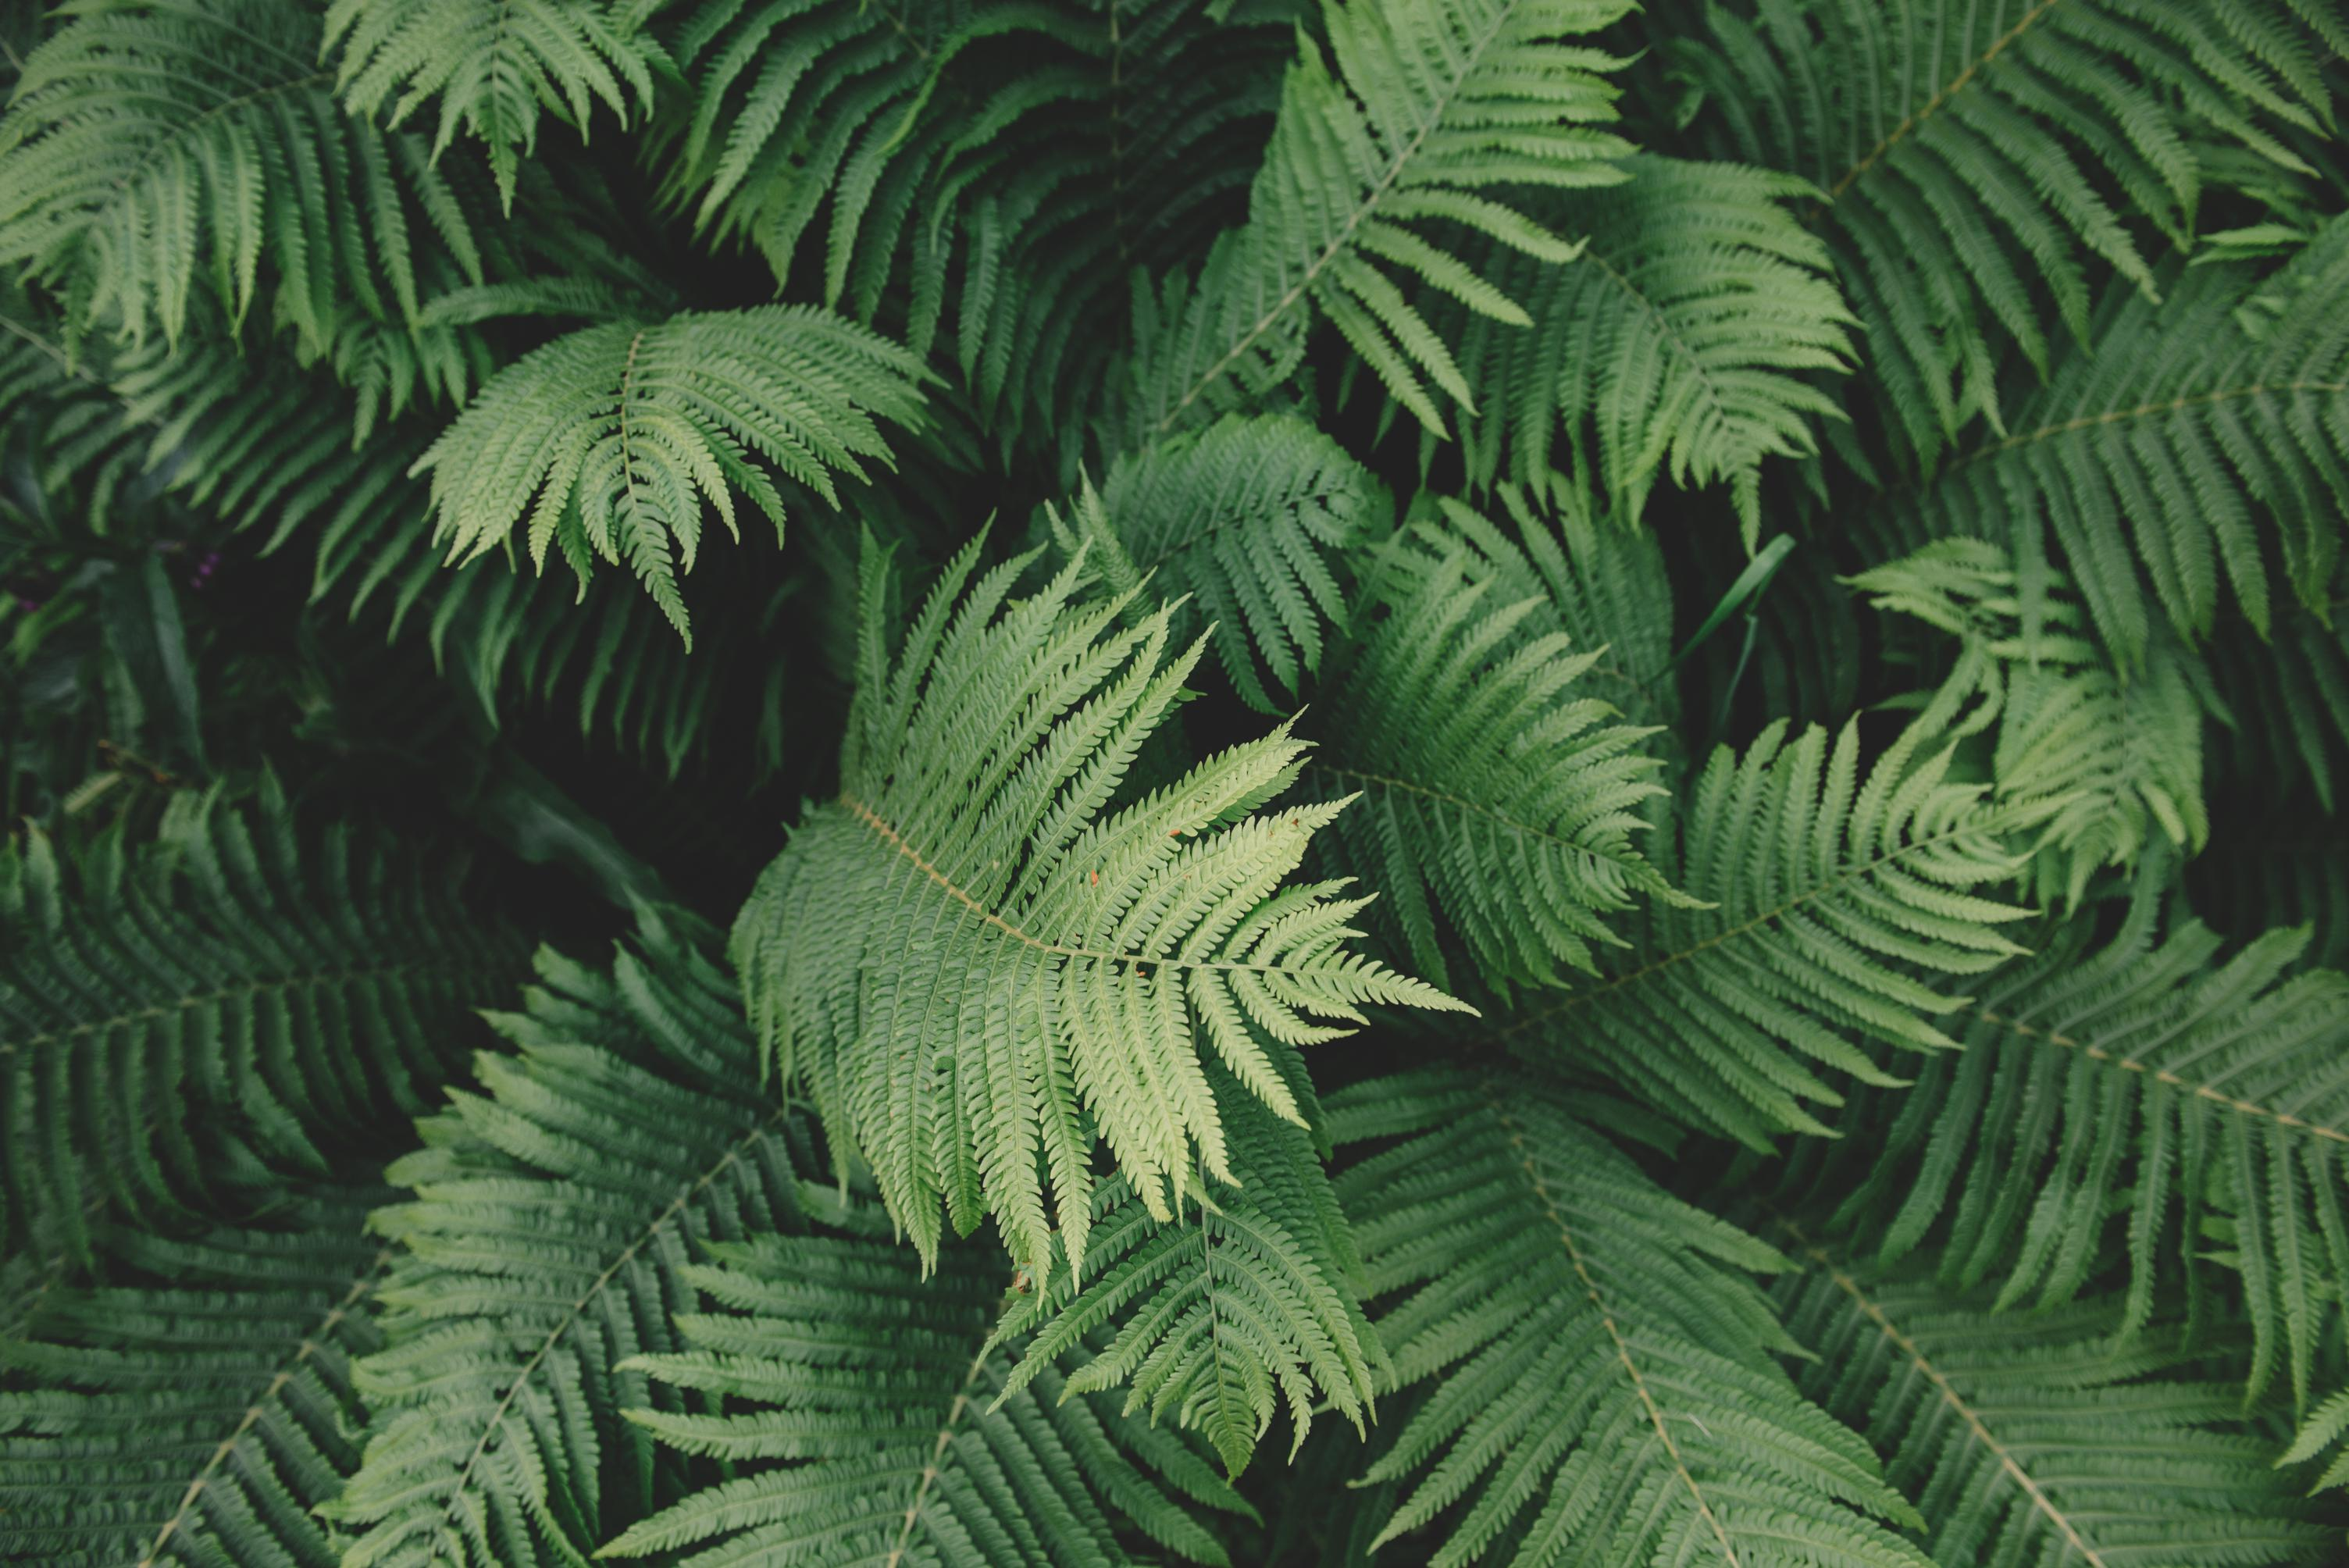
\includegraphics[width=.2\textwidth]{figures/chap4/photos/highshutter/2}}
    \subfigure[]{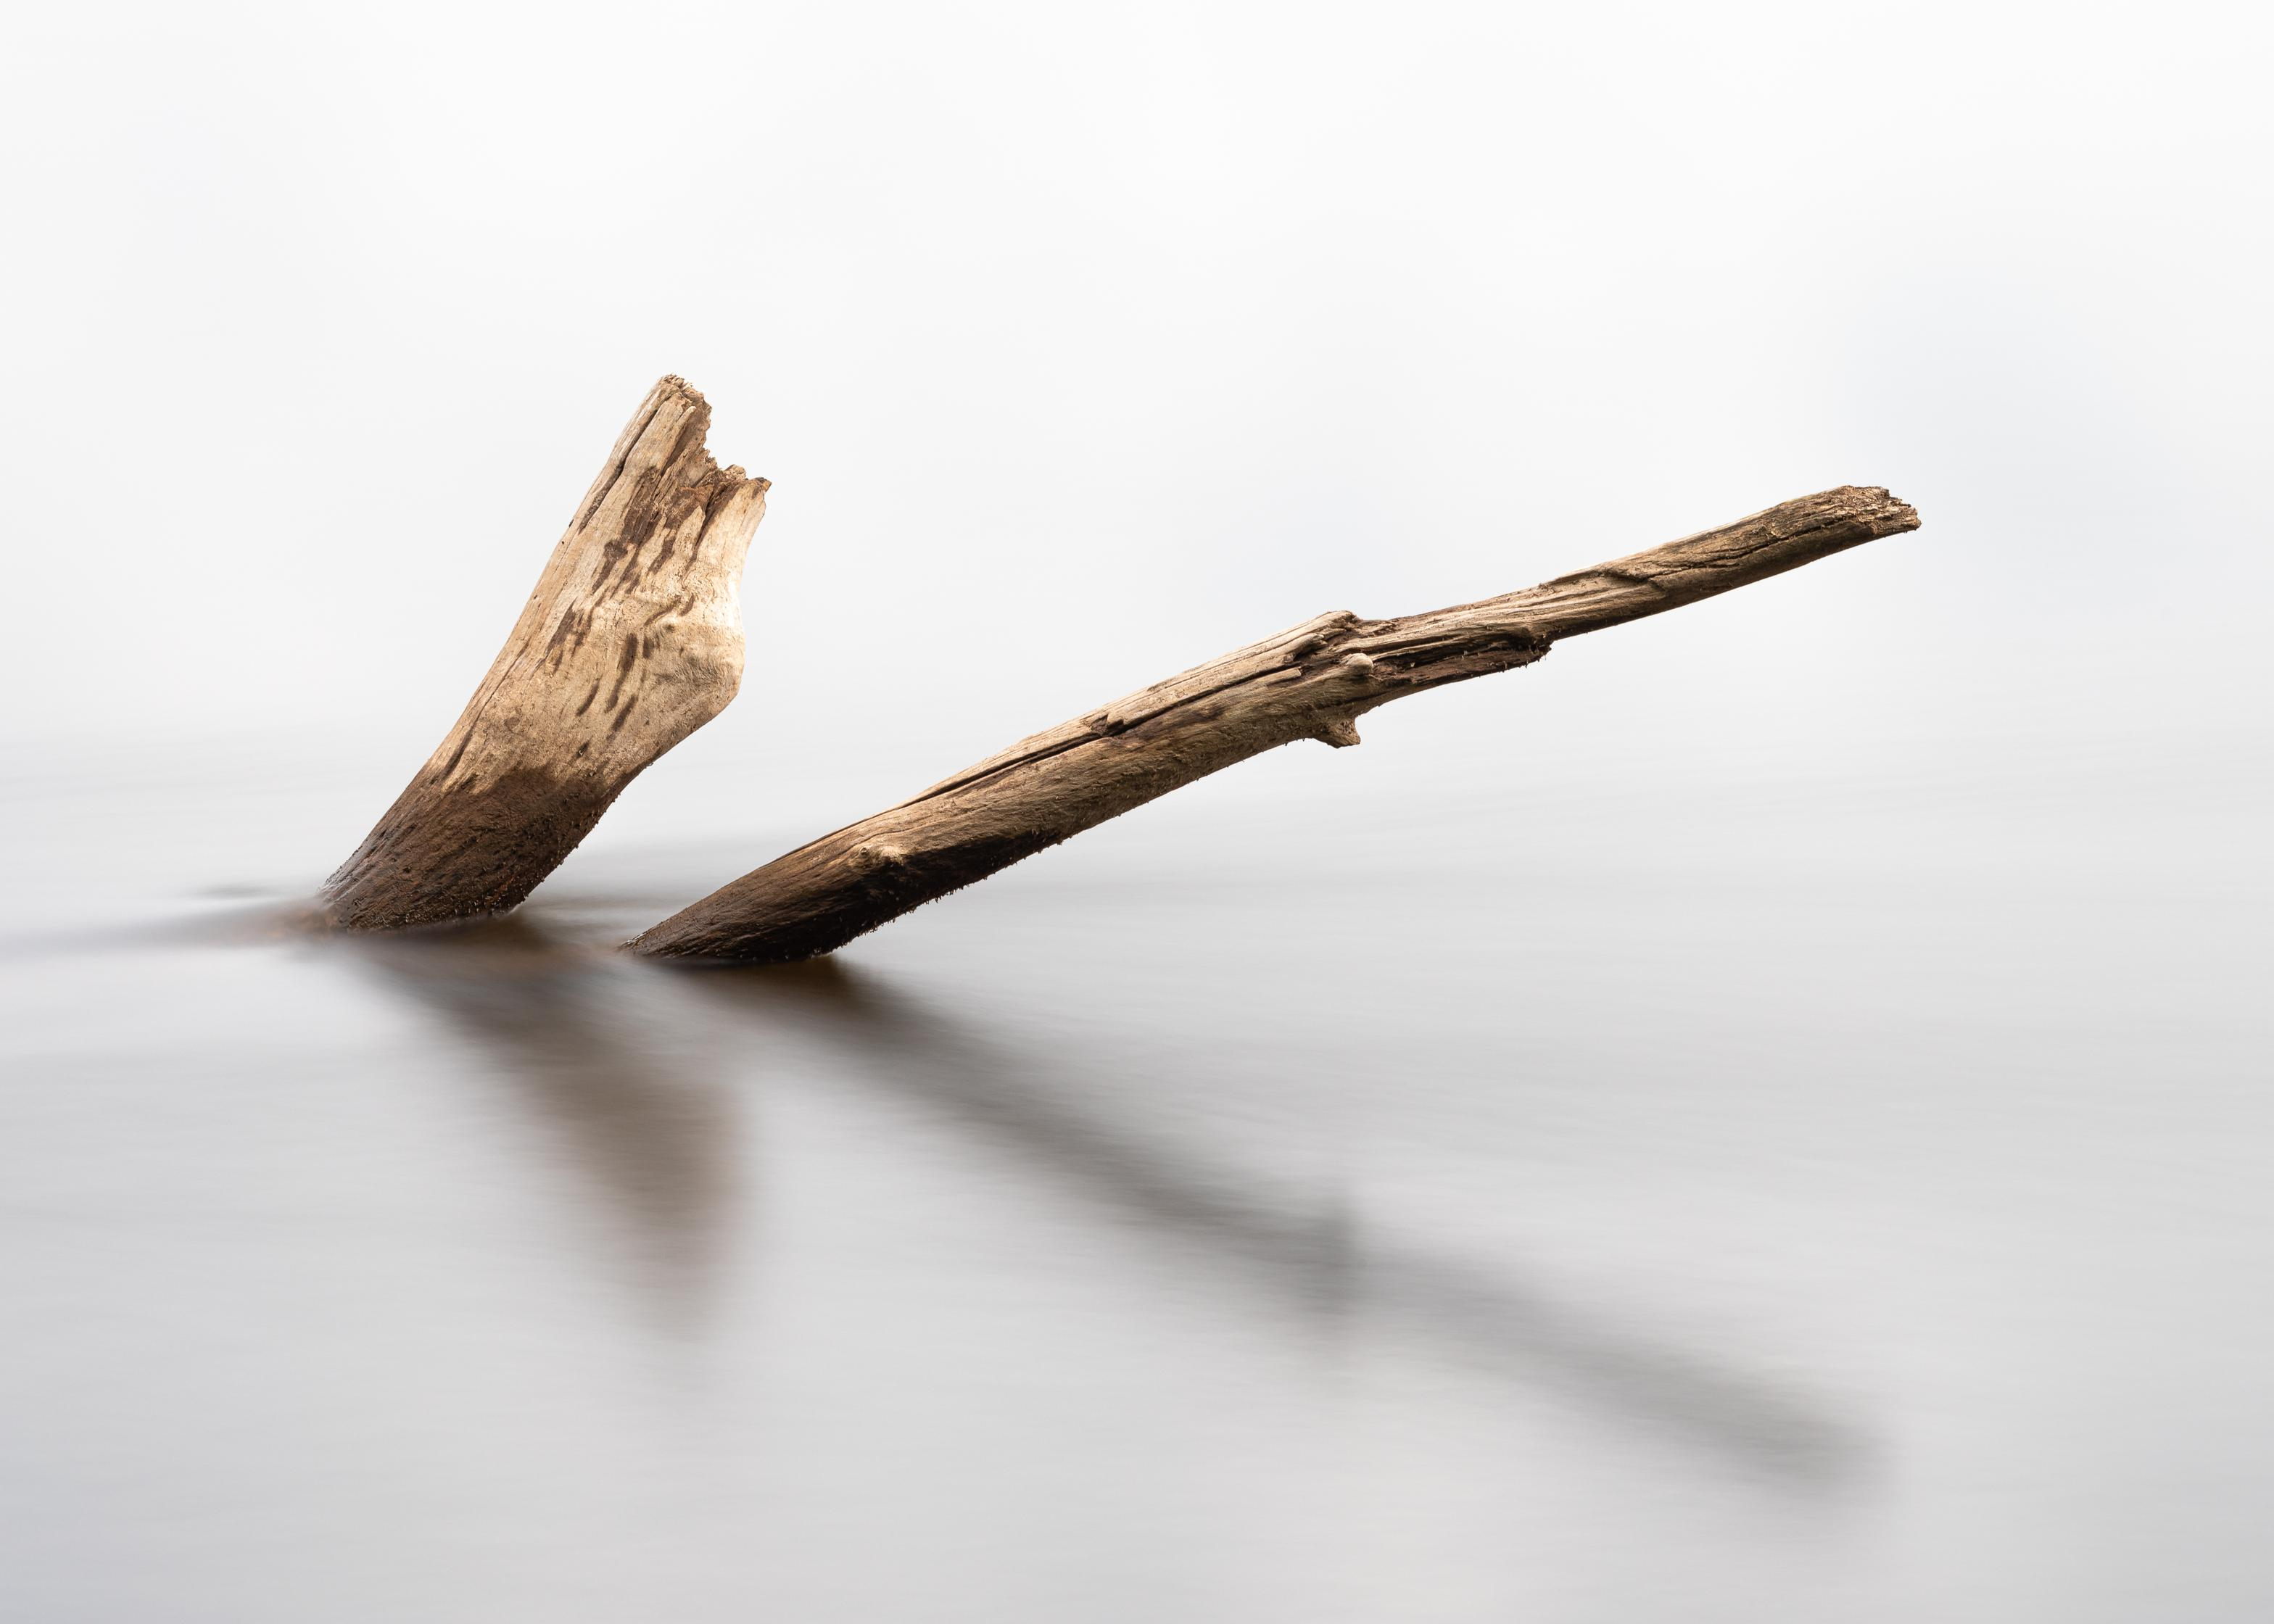
\includegraphics[width=.2\textwidth]{figures/chap4/photos/longexp/1}}
    \subfigure[]{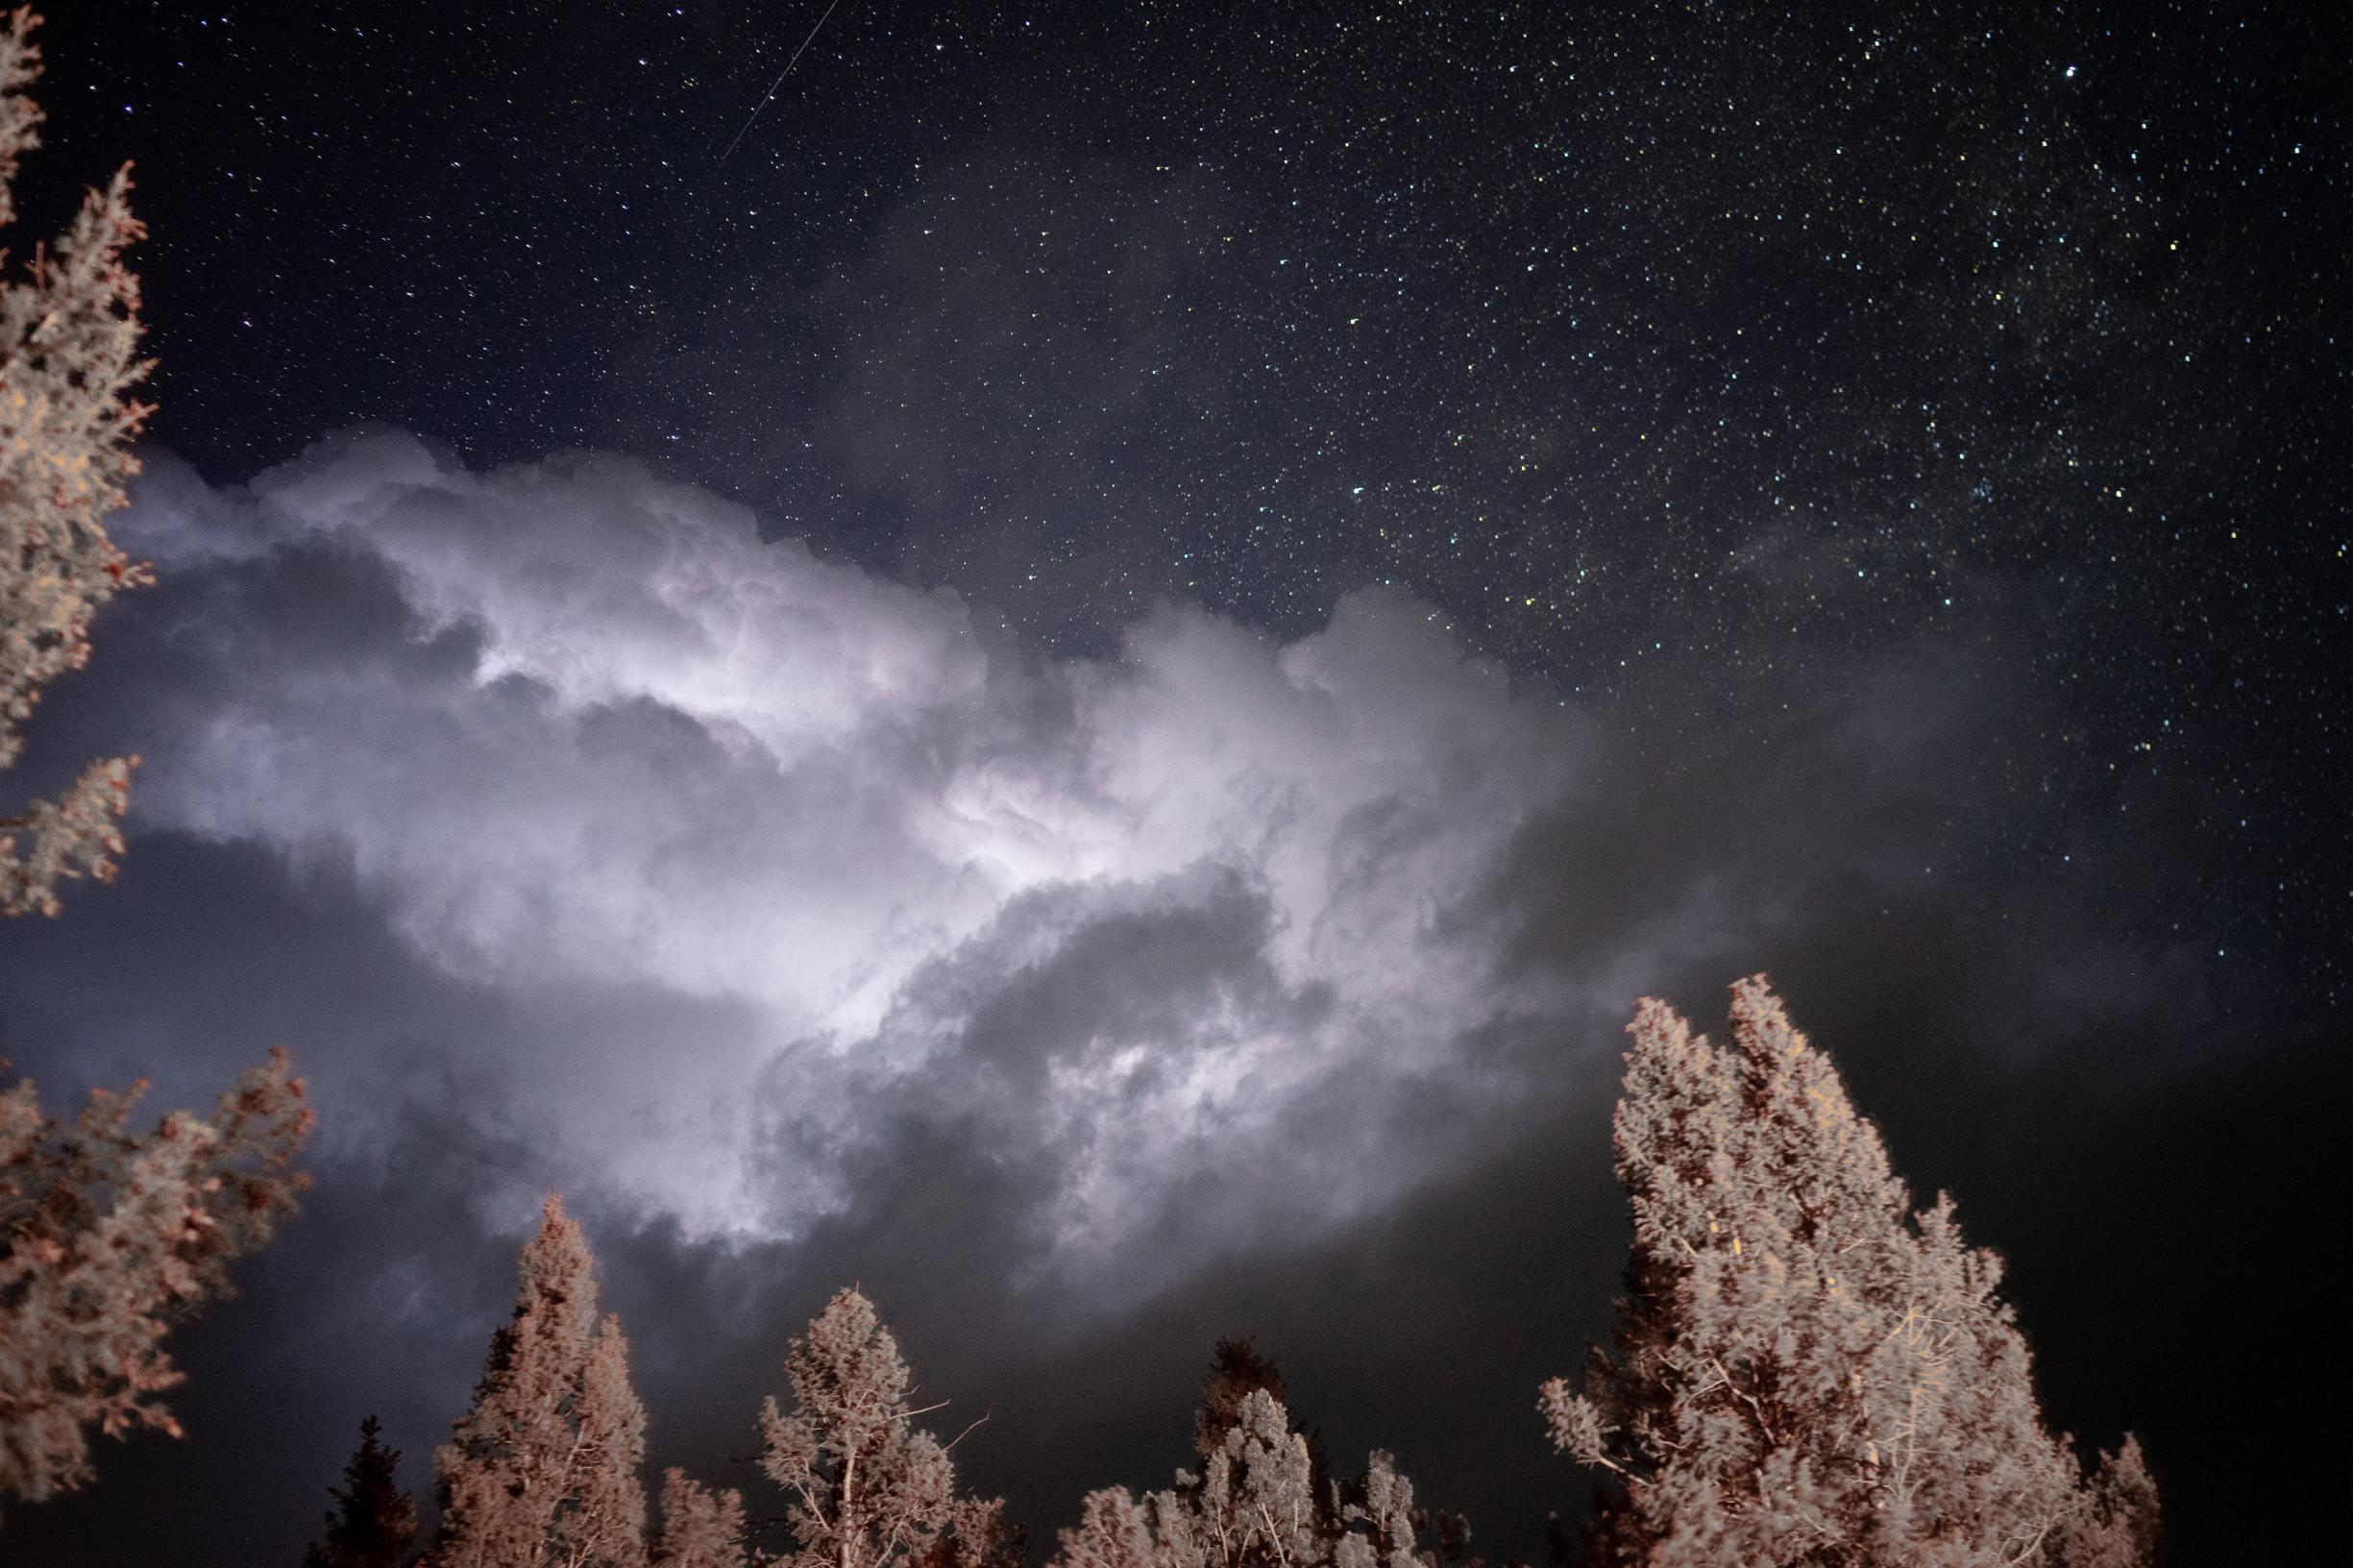
\includegraphics[width=.2\textwidth]{figures/chap4/photos/longexp/2}}    
    \caption{(a,b): Captures in fast $1/1000$ shutter speed setting, (c,d): Long exposured captures for 30''}
    \label{c4:fast_shutter_captures}
\end{figure}




%\begin{figure}[ht!]
%\centering  
%    \subfigure[DoF]{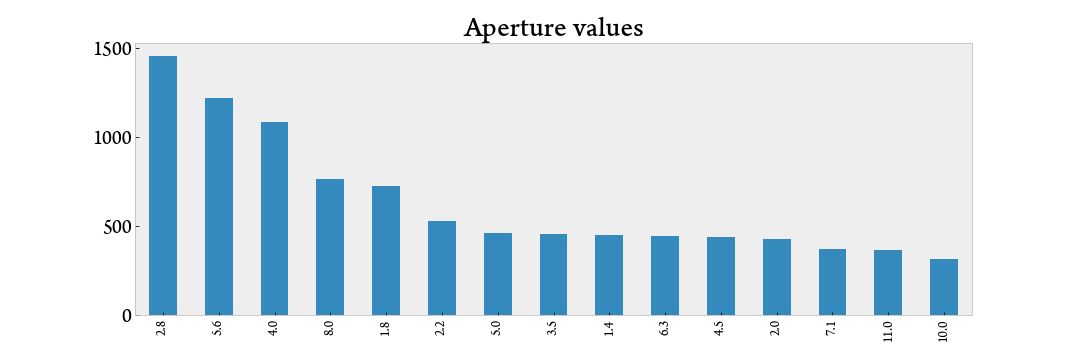
\includegraphics[width=.6\textwidth]{figures/chap4/exif/horizontal/aperture_values}}
%    \subfigure[ISO]{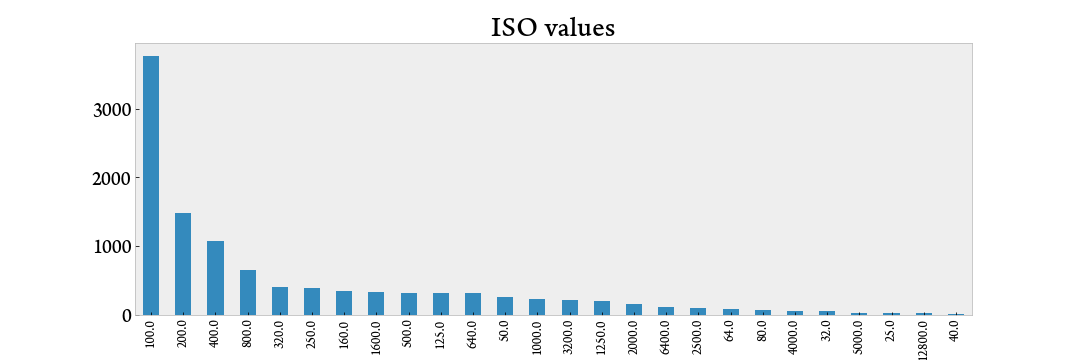
\includegraphics[width=.6\textwidth]{figures/chap4/exif/horizontal/iso_values}}
%\subfigure[Focal Length]{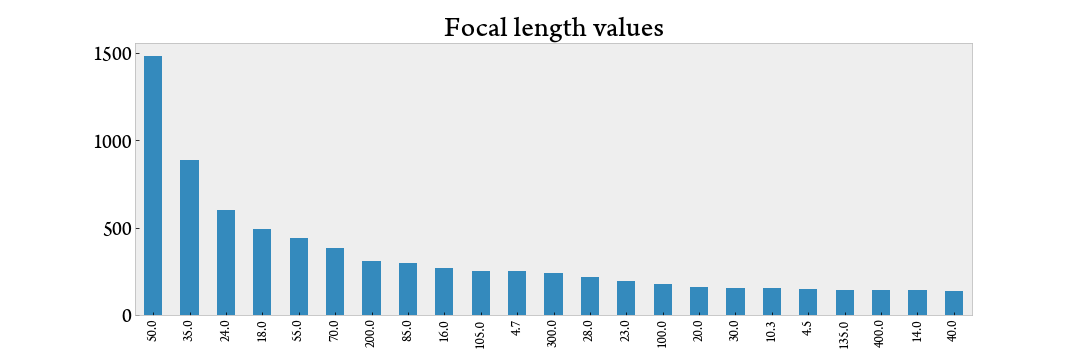
\includegraphics[width=.6\textwidth]{figures/chap4/exif/horizontal/focal_values}}
%    \subfigure[Exposure]{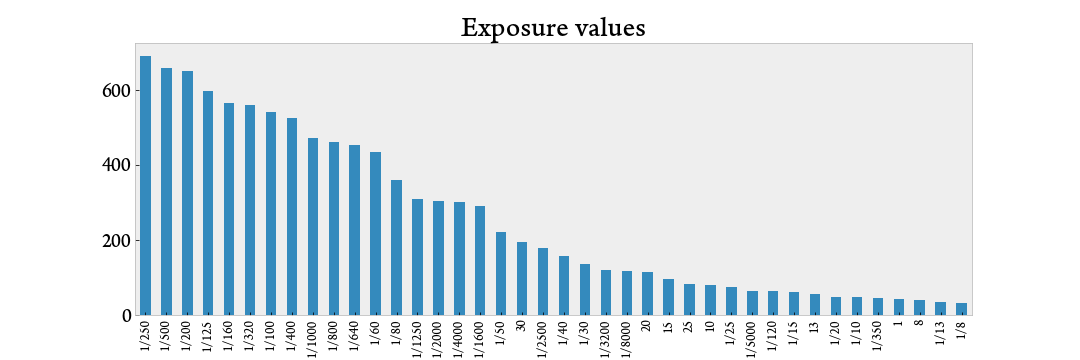
\includegraphics[width=.6\textwidth]{figures/chap4/exif/horizontal/exposure_values}}
%    \caption{Horizontal images DoF/ISO/Focal Length/Exposure value distribution}
%    \label{c4:horizontal_values_distribution}
%\end{figure}


%\begin{figure}[ht!]
%    \centering  
%    \subfigure[DoF]{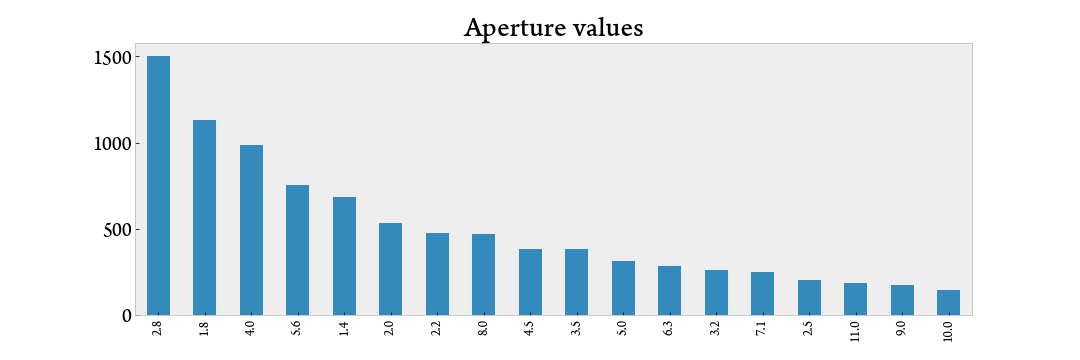
\includegraphics[width=.6\textwidth]{figures/chap4/exif/vertical/aperture_values}}
%    \subfigure[ISO]{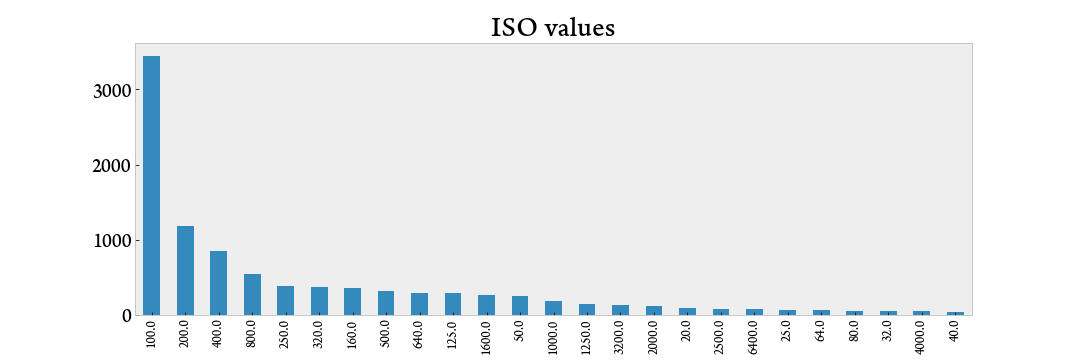
\includegraphics[width=.6\textwidth]{figures/chap4/exif/vertical/iso_values}}
%    \subfigure[Focal Length]{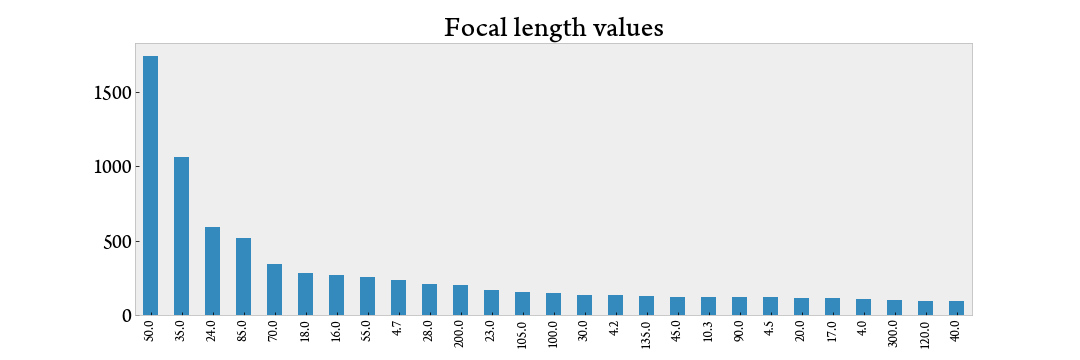
\includegraphics[width=.6\textwidth]{figures/chap4/exif/vertical/focal_values}}
%    \subfigure[Exposure]{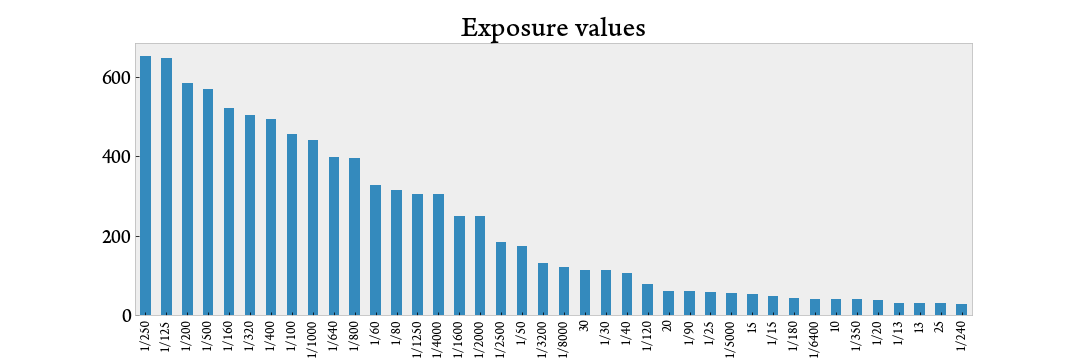
\includegraphics[width=.6\textwidth]{figures/chap4/exif/vertical/exposure_values}}    
%    \caption{Vertical images DoF/ISO/Focal Length/Exposure value distribution}
%    \label{c4:vertical_values_distribution}
%\end{figure}



\section{Data binning}
\label{c4:binning}

%% Binning
After data cleaning process, the quality of metadata were determined in terms of validity and consistency in order to carry through binning process. 
\textbf{Binning} is a method where instances are divided into discrete intervals known as \textit{bins}, based on a particular thresholding strategy applied on instance values.
\textit{Binning by frequency} is a method that matches continuous instance values  in bins, which correspond to a certain threshold range.


In theory, concerning photography and the related EXIF metadata, a specified range of values in a certain EXIF category, should justify a meaningfull photography style namely, e.g. a picture with ``bokeh'' has shallow depth of field and is captured with a low aperture value. Long exposure shots can be achieved when the shutter value is set in more than 1sec.

In general, there isn't a standard choice for the number of bins. In our case, we have created only 2 and 3 bins.
The binning strategy we structured is described in Table~\ref{c4:table_binning}. It originates from our empirical knowledge and also inspired from~\cite{laurence2018camera} as well.
More bins would not have contributed to the problem as it would be inappropriate to consider to create more segments.

For certain photography styles namely \textit{short/long exposures}(freezed/smoothed) and \textit{bokeh/focused}(shallow/deep DoF) is already difficult to characterise a photo in more than two bins as no/some/very \textbf{DoF/exposure}. Thus a binary label would be adequate to map and classify certain photography styles while a three class could work depending on the data distribution and photography styles related to the introduced ISO noise e.g. clean/grainy/noisy.


\begin{table}[!ht]
\centering
\begin{tabular}{c|c|c|c|}
\cline{2-4}
        & \multicolumn{3}{c|}{\textbf{Bins}}    \\ \cline{1-4}
        \multicolumn{1}{|l|}{\textbf{EXIF}}  & \textbf{0}       &  \textbf{1}       & \textbf{2}  \\ \cline{1-4}
        \multicolumn{1}{|l|}{Aperture (DoF)}            & (0,3.2)          &  [3.2,5.6]        & (5.6,]  \\ \cline{1-4}
        \multicolumn{1}{|l|}{Aperture Binary (DoF)}        & (0,3.5]          &  (3.5,]           & -  \\ \cline{1-4}
        \multicolumn{1}{|l|}{Focal Length}   & (0, 35mm]        &  (35mm,85mm]      & (85mm, )    \\ \cline{1-4}
        \multicolumn{1}{|l|}{Focal Length Binary}  & (0, 35mm]     &  (35mm,)          & -    \\ \cline{1-4}
        \multicolumn{1}{|l|}{ISO}            & (0,500)          &  [500,1800)       & [1800,]    \\ \cline{1-4}
        \multicolumn{1}{|l|}{ISO Binary}     & (0,500)          &  [500,)           & -    \\ \cline{1-4}
        \multicolumn{1}{|l|}{Exposure}       & (, 0'']              &  (0, 1/250]       & (1/250,)   \\ \cline{1-4}
\end{tabular}
\caption{Binning categories in EXIF dataset}
\label{c4:table_binning}
\end{table}

Elaborating on the table~\ref{c4:table_binning}, the ideal scenario is that bin \textbf{0} indicates a shallow depth of field for aperture settings, wide angle shots for focal length, low noise for ISO and long exposures, while bins \textbf{1} and \textbf{2}, indicate shots with deep or deeper DoF, narrow or more narrow angles, grainy or noisy shots and short exposured shots for each of the categories respectively.

%%%%%%%%%%%%%%%%%%%%%%%%%%%%%%%%%%%%%%%%%%%%%%%%%%%%%%%

\subsection{Uni-variate label distributions}
\label{c4:distributions}

The following figures visualize a second family of distributions, of the created labels based on binned EXIF values. Distribution for both photo orientations are shown in Figure~\ref{c4:all_distr}, images in horizontal orientation in Figure~\ref{c4:hor_distr} and images in vertical orientation in Figure~\ref{c4:ver_distr}.

\begin{figure}[ht!]
    \centering  
    \subfigure[Aperture]{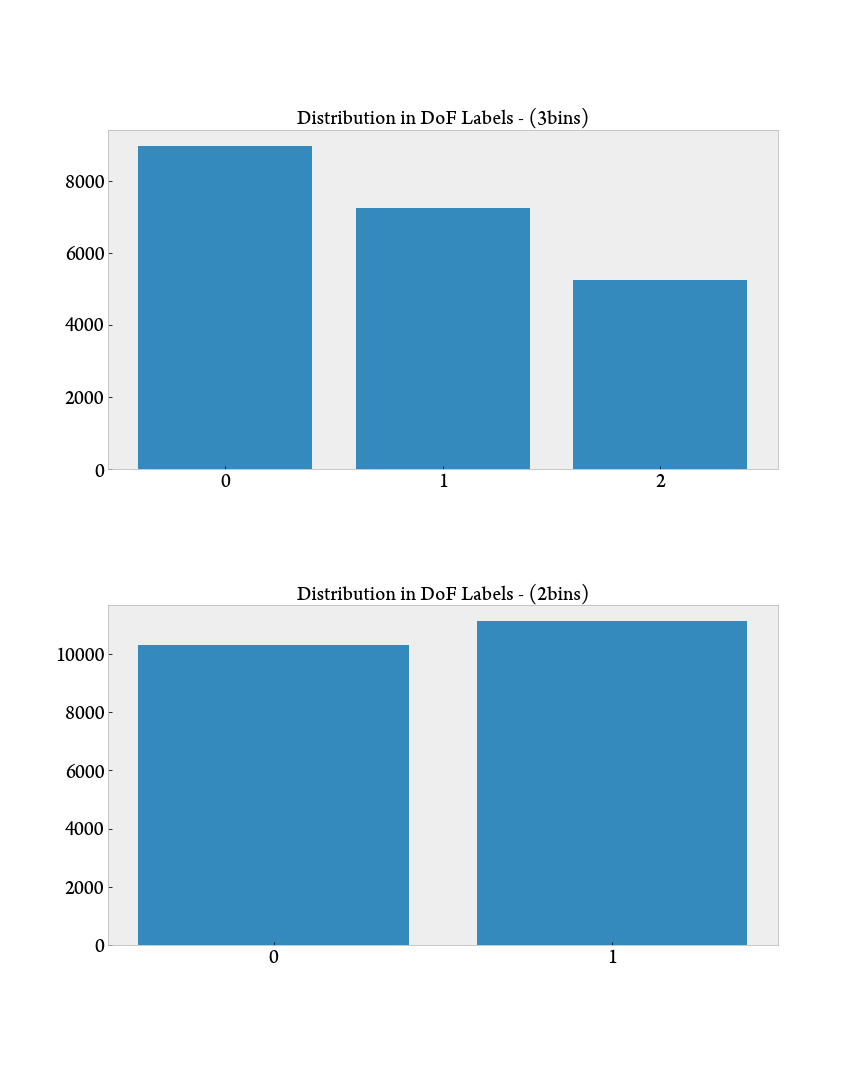
\includegraphics[width=.45\textwidth]{figures/chap4/exif/all/dof_bins}}
    \subfigure[ISO]{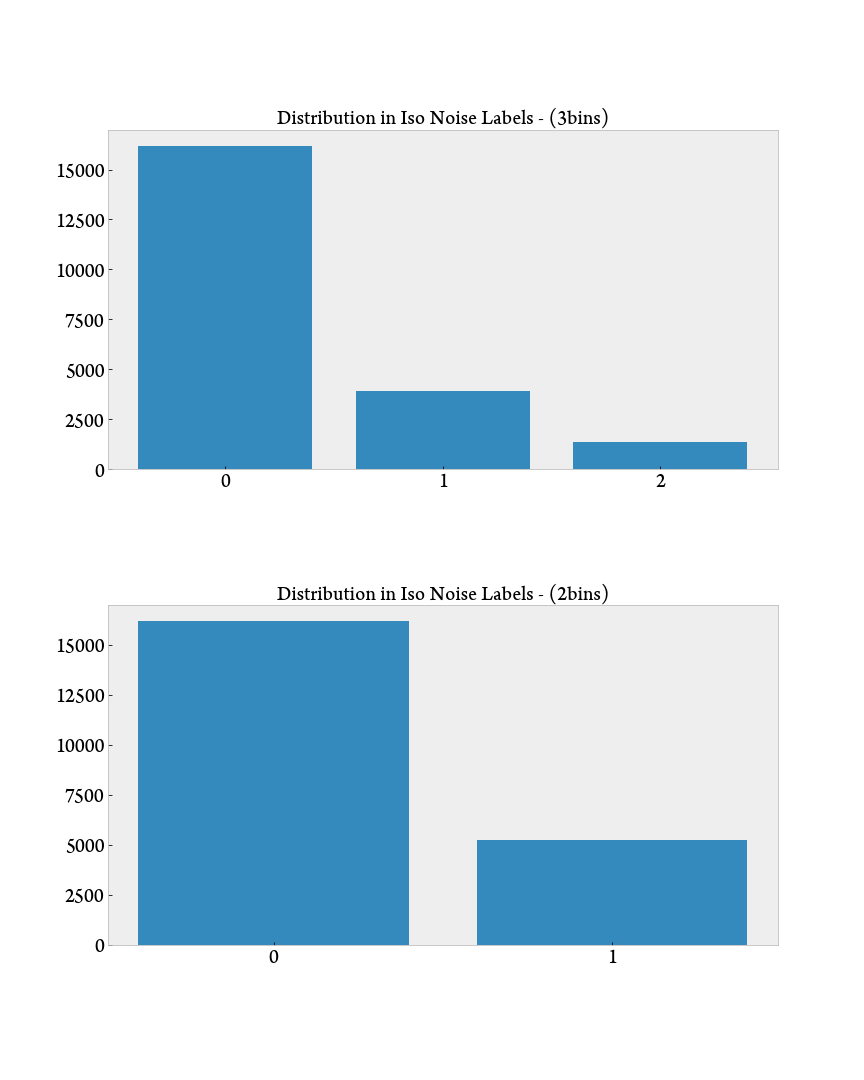
\includegraphics[width=.45\textwidth]{figures/chap4/exif/all/iso_bins}}
    \subfigure[Focal Length]{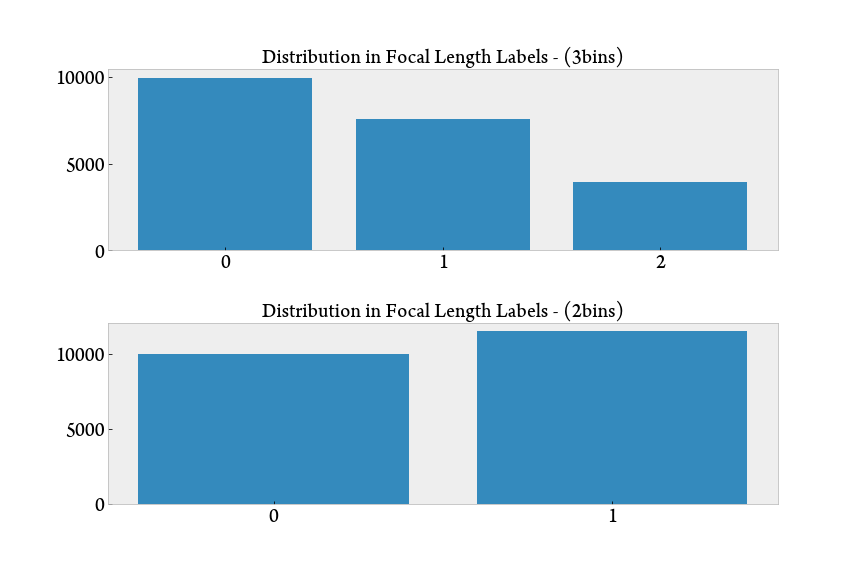
\includegraphics[width=.45\textwidth]{figures/chap4/exif/all/focal_length_bins}}
    \subfigure[Exposure]{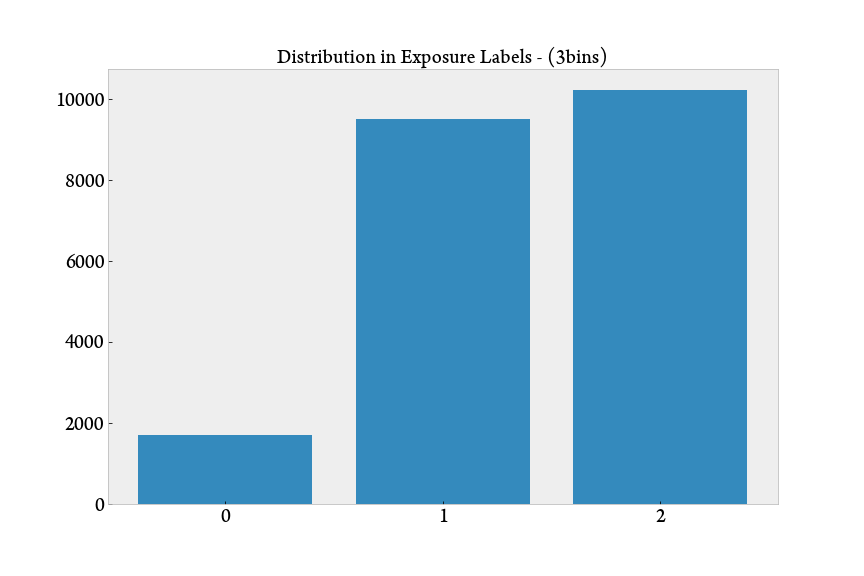
\includegraphics[width=.45\textwidth]{figures/chap4/exif/all/exposure_bins}}
    \caption{Horizontal$+$Vertical images for Aperture/ISO/Focal Length/Exposure label distribution}
    \label{c4:all_distr}
\end{figure}


\begin{figure}[ht!]
    \centering  
    \subfigure[Aperture]{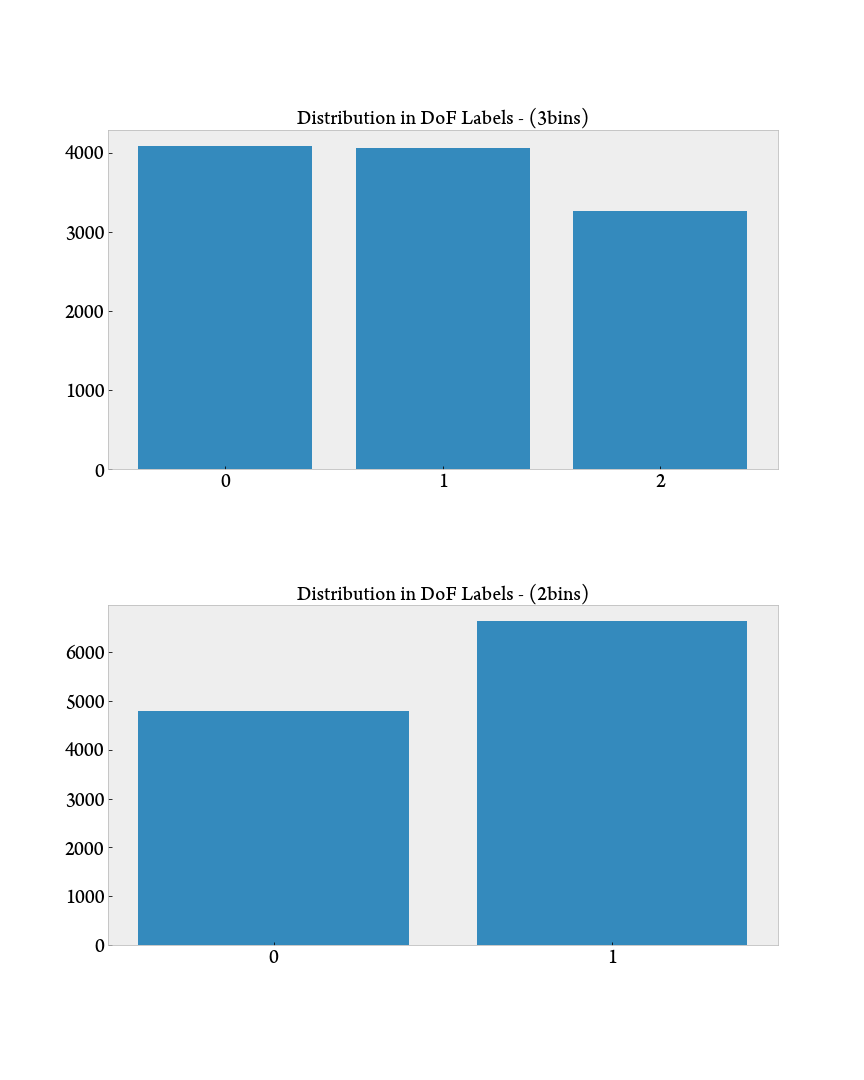
\includegraphics[width=.4\textwidth]{figures/chap4/exif/horizontal/dof_bins}}
    \subfigure[ISO]{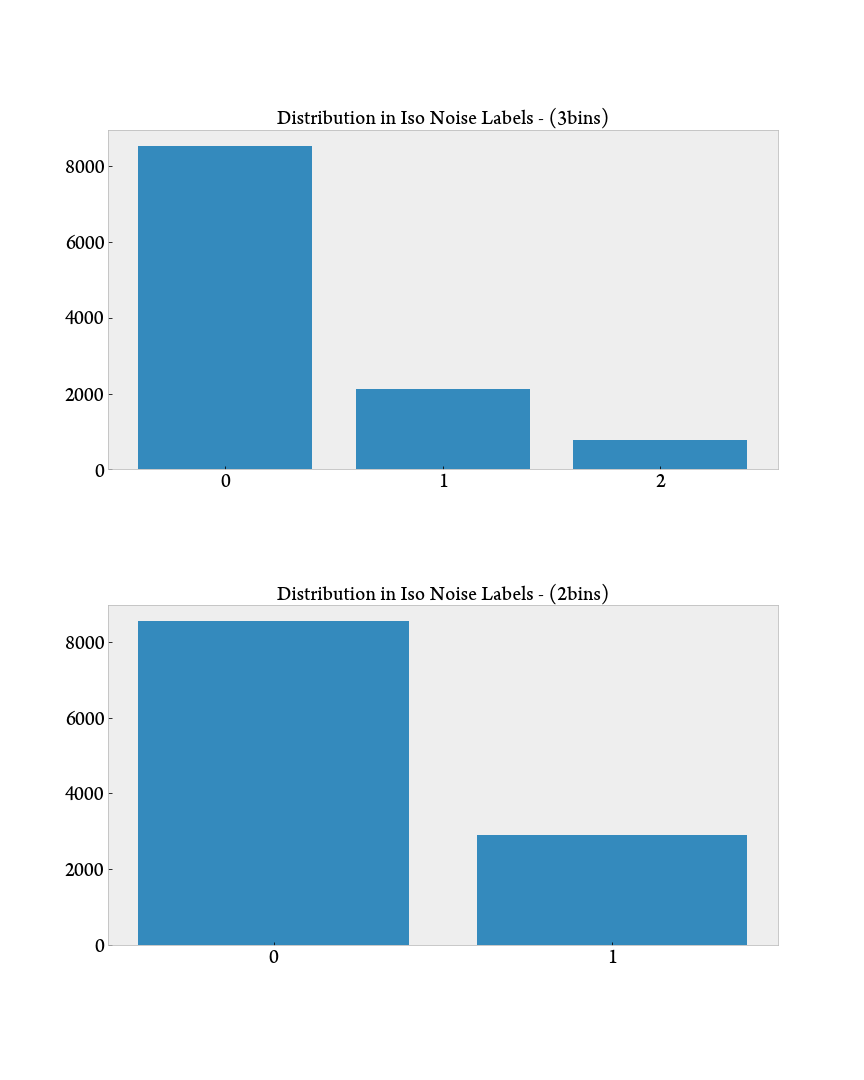
\includegraphics[width=.4\textwidth]{figures/chap4/exif/horizontal/iso_bins}}
    \subfigure[Focal Length]{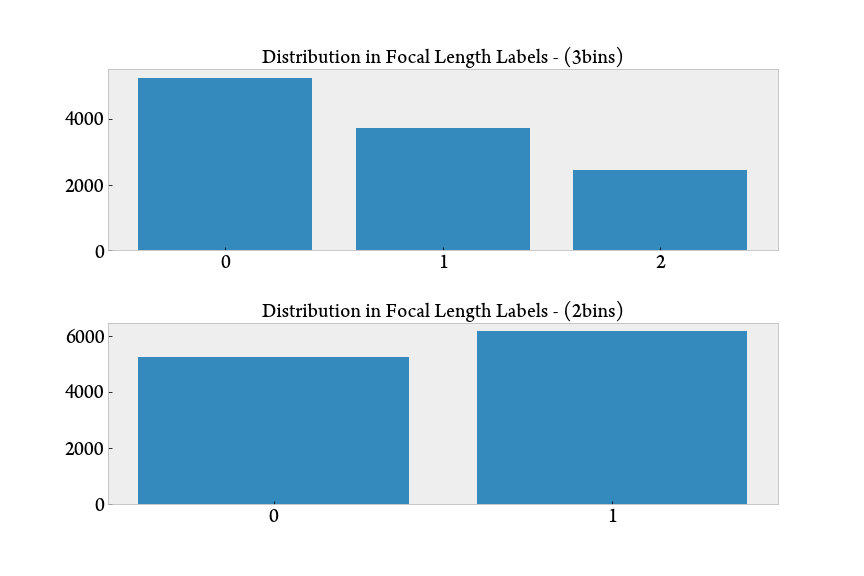
\includegraphics[width=.4\textwidth]{figures/chap4/exif/horizontal/focal_length_bins}}
    \subfigure[Exposure]{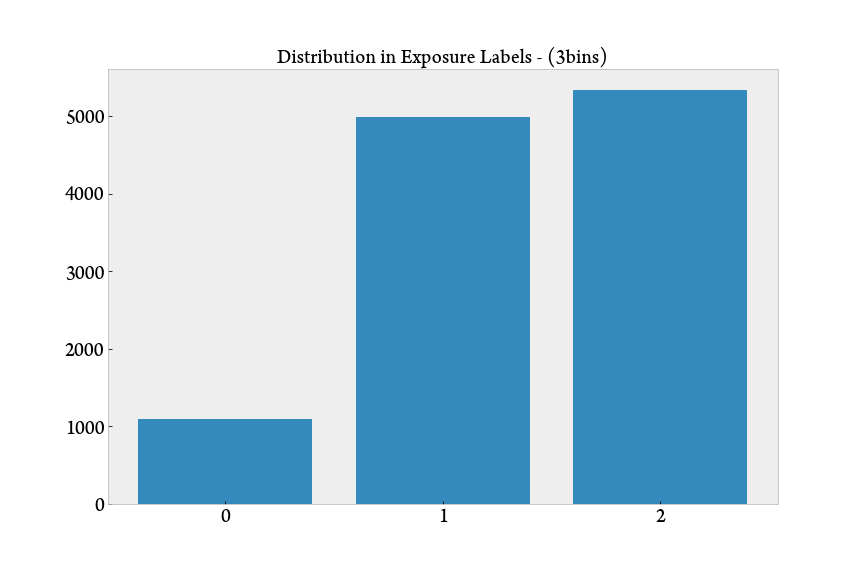
\includegraphics[width=.4\textwidth]{figures/chap4/exif/horizontal/exposure_bins}}    
    \caption{Horizontal images for Aperture/ISO/Focal Length/Exposure label distribution}
    \label{c4:hor_distr}
\end{figure}

\begin{figure}[ht!]
    \centering  
    \subfigure[Aperture]{\includegraphics[width=.45\textwidth]{figures/chap4/exif/vertical/dof_bins}}
    \subfigure[ISO]{\includegraphics[width=.45\textwidth]{figures/chap4/exif/vertical/iso_bins}}
    \subfigure[Focal Length]{\includegraphics[width=.45\textwidth]{figures/chap4/exif/vertical/focal_length_bins}}
    \subfigure[Exposure]{\includegraphics[width=.45\textwidth]{figures/chap4/exif/vertical/exposure_bins}}    
    \caption{Vertical images for Aperture/ISO/Focal Length/Exposure label distribution}
    \label{c4:ver_distr}
\end{figure}


By studying the distributions, we acquire substantial knowledge about the variability of bins existing in the same population.

The EXIF bins, that are skewed in one class and considered inappropriate as candidate labels, are the ISO and exposure. One would argue that there are plenty of samples to undersample from the majority class, but the contradiction could be that \textit{ISO} could have been post processed from a third party software before the picture is published and for \textit{exposure} normally even the human eye cannot detect distinct differences if a picture belong in bin \textbf{1} or \textbf{2}.

Concerning the distribution in \textbf{aperture} bins, is considered an ideal case to focus on, as it can be translated to an appealing photography style namely \textit{Bokeh}.
Bokeh effect is a famous and widely spread photography style. It is already artificially incorporated in most of the consumer smart-phone camera applications.  On the other hand, bokeh adds a softer and warm tone in a picture which is attractive to the users who share and publish content.

\section{Formulating the problem}
\label{c4:problem_formulation}

Combining the aforementioned visualised distributions with photography domain knowledge, we chose continue with aperture based bin, the one in two classes and consider it as a binary label to annotate the dataset.

As it has been mentioned in the previous section, an extra class for the current use case wouldn't have been supported qualitatively.

Finally the data set distribution led us to formulate a problem and define Bokeh photography style, to consider as the target class. Thus, we will attempt to create a binary classifier in order to learn and discriminate image with shallow and deep DoF.


\section{EXIF dataset - Data Sampling/Splitting}
\label{c4:exif_dataset}


In the previous section we showed that most of the camera settings appear to be more common than others.
For the selected use case, the EXIF based binary set for Bokeh style, is composed of $10,322$ samples for the low class and $11,123$ samples for the high class.
The most common methods to smooth class imbalance problems are oversampling and undersampling~\cite{japkowicz2002class}.
To tackle the imbalance problem we undersampled from the majority class as the Figure~\ref{c4:undersample} depicts. Undersampling is defined as to randomly remove examples from the majority class in order to balance the cardinality of minority class.

\begin{figure}[ht!]
    \centering  
    \includegraphics[width=.45\textwidth]{figures/chap4/undersampling}
    \caption{Undersampling strategy}
    \label{c4:undersample}
\end{figure}

Undersampling is applied for three datasets types as follows:
\begin{itemize}
 \item Horizontal$+$Vertical image orientantions with directly undersampling from the majority class
 \item Horizontal images, filtered out from the total samples and then undersampled the majority class
 \item Vertical images, in the same way
\end{itemize}

Table~\ref{c4:sampling_table} denotes the number of samples for the three dataset before and after undersampling.

\begin{table}[ht!]
\centering
\begin{tabular}{|c|c|c|c|c|c|c|}
\cline{1-7}
  & \multicolumn{3}{c|}{Unbalanced} & \multicolumn{3}{c|}{Balanced} \\ \cline{1-7} 
 Orientation  &   0    &   1    &  Total     &   0    &   1    &  Total     \\ \cline{1-7} 
H$+$V & \textbf{10322} & 11123 & 21445 & 10322 & 10322  &  20644 \\ \cline{1-7} 
Horizontal  & \textbf{4800} & 6629 & 11429 & 4800 & 4800 &  9600  \\ \cline{1-7} 
Vertical & 5522 & \textbf{4494}  & 10016 & 4494 & 4494 &  8988     \\ \cline{1-7} 
\end{tabular}
\caption{Dataset cardinalities before and after undersampling}
\label{c4:sampling_table}
\end{table}

Also figures~\ref{c4:all_sampling_labels},~\ref{c4:horizontal_sampling_labels} and~\ref{c4:vertical_sampling_labels} depict the cardinality of samples for each label before and after undersampling for all dataset types.

\begin{figure}[ht!]
    \centering  
    \subfigure[Unbalanced]{\includegraphics[width=.45\textwidth]{figures/chap4/exif/all/all_dof_unbalanced}}
    \subfigure[Balanced]{\includegraphics[width=.45\textwidth]{figures/chap4/exif/all/all_dof_balanced}}
    \caption{Horizontal$+$Vertical Unbalanced vs Balanced}
    \label{c4:all_sampling_labels}
\end{figure}

\begin{figure}[ht!]
    \centering  
    \subfigure[Unbalanced]{\includegraphics[width=.45\textwidth]{figures/chap4/exif/horizontal/horizontal_dof_unbalanced}}
    \subfigure[Balanced]{\includegraphics[width=.45\textwidth]{figures/chap4/exif/horizontal/horizontal_dof_balanced}}
    \caption{Horizontal Unbalanced vs Balanced}
    \label{c4:horizontal_sampling_labels}
\end{figure}

\begin{figure}[ht!]
    \centering  
    \subfigure[Unbalanced]{\includegraphics[width=.45\textwidth]{figures/chap4/exif/vertical/vertical_dof_unbalanced}}
    \subfigure[Balanced]{\includegraphics[width=.45\textwidth]{figures/chap4/exif/vertical/vertical_dof_balanced}}
    \caption{Vertical Unbalanced vs Balanced}
    \label{c4:vertical_sampling_labels}
\end{figure}


Finally each one of the datasets has been split by 80/10/10 ratio in balanced train, validation and test sets.

\subsection{EXIF dataset - image samples}
\label{c4:exif_samples}

Motivated by problem formulation in Section~\ref{c4:problem_formulation}, samples of \textbf{EXIF} dataset, binned in low and high classes of depth of field are provided in Figures~\ref{c4:all_low_class_samples}-\ref{c4:vertical_high_class_samples}.



Investigating the sampled photos, we are looking for pictures with noticeable shallow DoF level in low class Figures~\ref{c4:all_low_class_samples},~\ref{c4:horizontal_low_class_samples},~\ref{c4:vertical_low_class_samples} where the subject should stand-out from the background.

% all
\begin{figure}[ht!]
    \centering  
    \subfigure{\includegraphics[width=.2\textwidth]{figures/chap4/exif/all/samples/0/1}}
    \subfigure{\includegraphics[width=.2\textwidth]{figures/chap4/exif/all/samples/0/2}}
    \subfigure{\includegraphics[width=.2\textwidth]{figures/chap4/exif/all/samples/0/3}}
    \subfigure{\includegraphics[width=.2\textwidth]{figures/chap4/exif/all/samples/0/4}}
    \caption{EXIF dataset - Horizontal$+$Vertical sample images low(0) class - shallow DoF}
    \label{c4:all_low_class_samples}
\end{figure}


% Horizontal 
\begin{figure}[h!]
    \centering  
    \subfigure{\includegraphics[width=.2\textwidth]{figures/chap4/exif/horizontal/samples/0/1}}
    \subfigure{\includegraphics[width=.2\textwidth]{figures/chap4/exif/horizontal/samples/0/2}}
    \subfigure{\includegraphics[width=.2\textwidth]{figures/chap4/exif/horizontal/samples/0/3}}
    \subfigure{\includegraphics[width=.2\textwidth]{figures/chap4/exif/horizontal/samples/0/4}}
    \caption{EXIF dataset - Horizontal sample images low(0) class - shallow DoF}
    \label{c4:horizontal_low_class_samples}
\end{figure}

% Vertical

\begin{figure}[h!]
    \centering  
    \subfigure{\includegraphics[width=.15\textwidth]{figures/chap4/exif/vertical/samples/0/1}}
    \subfigure{\includegraphics[width=.15\textwidth]{figures/chap4/exif/vertical/samples/0/2}}
    \subfigure{\includegraphics[width=.15\textwidth]{figures/chap4/exif/vertical/samples/0/3}}
    \subfigure{\includegraphics[width=.15\textwidth]{figures/chap4/exif/vertical/samples/0/4}}
    \caption{EXIF dataset - Horizontal sample images low(0) class - shallow DoF}
    \label{c4:vertical_low_class_samples}
\end{figure}


While for pictures in Figures~\ref{c4:all_high_class_samples},~\ref{c4:horizontal_high_class_samples},~\ref{c4:vertical_high_class_samples} annotated in high class the DoF should be deep enough that the horizon should not be separated from the main subject.

\begin{figure}[h!]
    \centering  
    \subfigure{\includegraphics[width=.2\textwidth]{figures/chap4/exif/all/samples/1/1}}
    \subfigure{\includegraphics[width=.2\textwidth]{figures/chap4/exif/all/samples/1/2}}
    \subfigure{\includegraphics[width=.2\textwidth]{figures/chap4/exif/all/samples/1/3}}
    \subfigure{\includegraphics[width=.2\textwidth]{figures/chap4/exif/all/samples/1/4}}
    \caption{EXIF dataset - Horizontal$+$Vertical sample images high(1) class - deep DoF}
    \label{c4:all_high_class_samples}
\end{figure}

\begin{figure}[h!]
    \centering  
    \subfigure{\includegraphics[width=.2\textwidth]{figures/chap4/exif/horizontal/samples/1/1}}
    \subfigure{\includegraphics[width=.2\textwidth]{figures/chap4/exif/horizontal/samples/1/2}}
    \subfigure{\includegraphics[width=.2\textwidth]{figures/chap4/exif/horizontal/samples/1/3}}
    \subfigure{\includegraphics[width=.2\textwidth]{figures/chap4/exif/horizontal/samples/1/4}}

    \caption{EXIF dataset - Horizontal sample images high(1) class - deep DoF}
    \label{c4:horizontal_high_class_samples}
\end{figure}

\begin{figure}[h!]
    \centering  
    \subfigure{\includegraphics[width=.15\textwidth]{figures/chap4/exif/vertical/samples/1/1}}
    \subfigure{\includegraphics[width=.15\textwidth]{figures/chap4/exif/vertical/samples/1/2}}
    \subfigure{\includegraphics[width=.15\textwidth]{figures/chap4/exif/vertical/samples/1/3}}
    \subfigure{\includegraphics[width=.15\textwidth]{figures/chap4/exif/vertical/samples/1/4}}
    \caption{EXIF dataset - Horizontal sample images high(1) class - deep DoF}
    \label{c4:vertical_high_class_samples}
\end{figure}

By observing the samples, there are pictures where they seemed to be correctly categorized and DoF escalation makes sense. On the other hand, there are several cases where ``noise'' is introduced in bins, which is not due to faulty categorization but due to photography circumstances.
For example a picture with very low aperture setting can be used to produce a ``bokeh'' effect, but can also be used in night photography or even in daily photography when the subject is completely focused and occupies most of the frame's surface. The latter cases are met in the following figures and are considered as introduced noise.

\section{DoF Dataset - Manual Annotation}
\label{c4:dof_dataset}

We have created an \textbf{EXIF} based dataset, which was utilised to train a visual classifier in shallow and deep DoF content pictures. We were expecting that the induced noise can adversary affect the model training performance and classification capability. After attempting to train a number of different classifiers, results of the evaluation are presented in the next chapter, we did not observe any substantial performance and overall poor results.
Hence, we concluded that EXIF based data set, failed to reflect ``bokeh'' in pictures and is not considered appropriate to create a strong enough classifier to assess a certain photography style.

Our main concern, in order to effectively tackle the problem, is to construct a carefully annotated dataset, utilising domain knowledge.
We started from scratch and focused only on horizontal images where we carefully annotated a total of 1200 samples, equally balanced for the two classes. 
We split it in train, validation and test sets by 560/140/500 samples respectively.
One may argue for the uneven ratio split size between training/validation and testing sets. We chose a fairly large amount of test set in order to acquire more accurate posterior estimations of the classifier, since we delve into a task with limited or any prior knowledge.
Annotated image samples are shown in figures~\ref{c4:dof_horizontal_low_class_samples} and~\ref{c4:dof_horizontal_high_class_samples}.


% Horizontal 
\begin{figure}[h!]
    \centering  
    \subfigure{\includegraphics[width=.2\textwidth]{figures/chap4/dof/horizontal/0/1}}
    \subfigure{\includegraphics[width=.2\textwidth]{figures/chap4/dof/horizontal/0/2}}
    \subfigure{\includegraphics[width=.2\textwidth]{figures/chap4/dof/horizontal/0/3}}
    \subfigure{\includegraphics[width=.2\textwidth]{figures/chap4/dof/horizontal/0/4}}
    \caption{DoF dataset - Horizontal sample images low(0) class - shallow DoF}
    \label{c4:dof_horizontal_low_class_samples}
\end{figure}


\begin{figure}[ht!]
    \centering  
    \subfigure{\includegraphics[width=.2\textwidth]{figures/chap4/dof/horizontal/1/1}}
    \subfigure{\includegraphics[width=.2\textwidth]{figures/chap4/dof/horizontal/1/2}}
    \subfigure{\includegraphics[width=.2\textwidth]{figures/chap4/dof/horizontal/1/3}}
    \subfigure{\includegraphics[width=.2\textwidth]{figures/chap4/dof/horizontal/1/4}}
    \caption{DoF dataset - Horizontal sample images high(1) class - deep DoF}
    \label{c4:dof_horizontal_high_class_samples}
\end{figure}

In the next chapter, we provide an extended description about the methodology we followed to construct a range of deep learning classifier. In addition, we present an active learning framework that will help us to indicate the most informative unlabelled samples to include in the training set in order maximize the model performance and reduce annotation costs in time.
